\documentclass[12pt, twoside]{report}
\usepackage[a4paper,left=2cm, right=2cm, top=3cm,bottom=2cm]{geometry}
\usepackage[utf8]{inputenc}

\usepackage[english]{babel}
\usepackage{amsmath}
\usepackage{graphicx}
\usepackage{textcomp}
\usepackage{parskip}
\usepackage[colorinlistoftodos]{todonotes}
\usepackage{csquotes}
\usepackage{float}
\usepackage[backend=biber,style=ieee]{biblatex}
\usepackage{hyperref}
\usepackage{graphicx}
\usepackage{epsfig}
\usepackage{caption}
\usepackage{ragged2e}
\usepackage{subcaption}
\usepackage[singlespacing]{setspace}
\usepackage{hyperref}
\usepackage[utf8]{inputenc}
\usepackage[backend=biber,style=ieee]{biblatex}

\usepackage{biblatex}

%\addbibresource{friedt.bib}
\addbibresource{OCT_ref.bib}
\setlength {\marginparwidth }{2cm} 

%Chapter and name in the same line
\usepackage{titlesec}
\titleformat{\chapter}[hang] 
{\normalfont\huge\bfseries}{\chaptertitlename\ \thechapter:}{1em}{} 

\titleformat{\chapter}[display]
  {\normalfont\bfseries}{}{0pt}{\Huge}
  

\usepackage{listings}
\definecolor{mygreen}{rgb}{0,0.6,0}
\definecolor{mygray}{rgb}{0.5,0.5,0.5}
\definecolor{mymauve}{rgb}{0.58,0,0.82}
\lstset{ 
  language=Octave,
  backgroundcolor=\color{white},
  basicstyle=\footnotesize,       
  breakatwhitespace=false,         
  breaklines=true,
  captionpos=b,
  commentstyle=\color{mygreen},    
  deletekeywords={...},         
  escapeinside={\%*}{*)},        
  extendedchars=false,              
  frame=single,	                  
  keepspaces=true,                 
  keywordstyle=\color{blue},                       
  morekeywords={*,...},          
  numbers=left,                    
  numbersep=5pt,                   
  numberstyle=\tiny\color{mygray}, 
  rulecolor=\color{black},        
  showspaces=false,               
  showstringspaces=false,        
  showtabs=false,                
  stepnumber=1,                    
  stringstyle=\color{mymauve},     
  tabsize=2,	                   
  title=\lstname                   
}




\begin{document}


\lstset{language=Octave}
\begin{titlepage}

\newcommand{\HRule}{\rule{\linewidth}{0.5mm}}
\center 

\textsc{\LARGE Université Bourgogne Franche-Comté}\\[1.5cm] 
\textsc{\Large Master 2 in Smart Integrated Systems}\\[0.5cm] 

\HRule \\[0.4cm]
{ \huge \bfseries Report TP 3D Computer Vision}\\[0.4cm] 
\HRule \\[1.5cm]


\includegraphics[scale=0.3]{logo_ubfc.png}\\[1cm]

\begin{center}
\begin{tabular}{ c   |   c } 
   
    Grover ARUQUIPA & \normalsize \href{mailto:grover.aruquipa@femto-st.fr}{grover \textunderscore aruquipa \textunderscore @femto-st.fr}
    %Opcion 2:
    %ARUQUIPA Grover & \normalsize \href{mailto:grover.grover_aruquipa_aruquipa@edu.univ-fcomte.fr}{grover.grover \textunderscore aruquipa \textunderscore aruquipa@edu.univ-fcomte.fr}\\
    %RIVERA Carlos &  \normalsize \href{mailto:carlos_manuel.rivera_aguilar@edu.univ-fcomte.fr}{carlos\textunderscore manuel.rivera\textunderscore aguilar@edu.univ-fcomte.fr}
\end{tabular}
\end{center}

\vfill
{\large \today}\\[1cm] 
\vfill 

\end{titlepage}
 

%\thispagestyle{empty}
%\tableofcontents
%\listoffigures
\pagebreak



\pagebreak



    


\chapter{Session 1}
In this section we proceeded to perform the calibration of the camera in order to obtain the intrinsic parameters that are a fundamental part to perform the homography and pose estimation calculations.\\
The implementation of this section is available in the attached repository at\footnote{\href{https://github.com/GroverAruquipa/3D_Computer_m2}{$https://github.com/GroverAruquipa/3D_Computer_m2$}}.
\begin{enumerate}
    \item \textbf{Recall what is the purpose of camera calibration and its resolution steps.}\\
    To carry out the calibration, a series of steps must be followed, firstly, it seeks to use a mosaic with different grids, which helps to identify the number of corners (knowing the size of each grid), it proceeds to find samples through of different poses of the camera, later through these corners an optimization process is carried out through which the camera calibration methods are obtained.
    \item{\textbf{The matrix K presented in equation 1 is not complete, what is missing for the model
screening is complete?}}
    Depending on the steps indicated in the master classes, it is observed that the calibration matrix has the necessary parameters, on the other hand, in Eq. 1, it seemed that the identity matrix plus the vector column 0 is not taken into account, according to Eq. 2 .
    \item{\textbf{Before performing the camera calibration, list the different concrete applications in the
case where:}}
    \subitem{\textbf{K, cTo, oP Knowns :} Used for Point Estimation.}
        \subitem{\textbf{p, P Knowns :} Used for Calibration or find the intrinsic parameters or the homography matrix.}
            \subitem{\textbf{p, K, cTo Knowns :} Used 3D reconstruction.}
    \item{\textbf{Combien d’images allez-vous acqu´erir pour effectuer l’´etalonnage de la cam´era ?}}\\
    According to the equations, at least three parallel images are needed for a stereo camera, at least 2 for each lens, but regarding the state of the art, the use of more than 20 images at different angles and perspectives is recommended in order to improve the precision based on uncertainty.
    
    \item \textbf{Perform the calibration of the acquired images.}

    \begin{figure}[H]
    \centering
    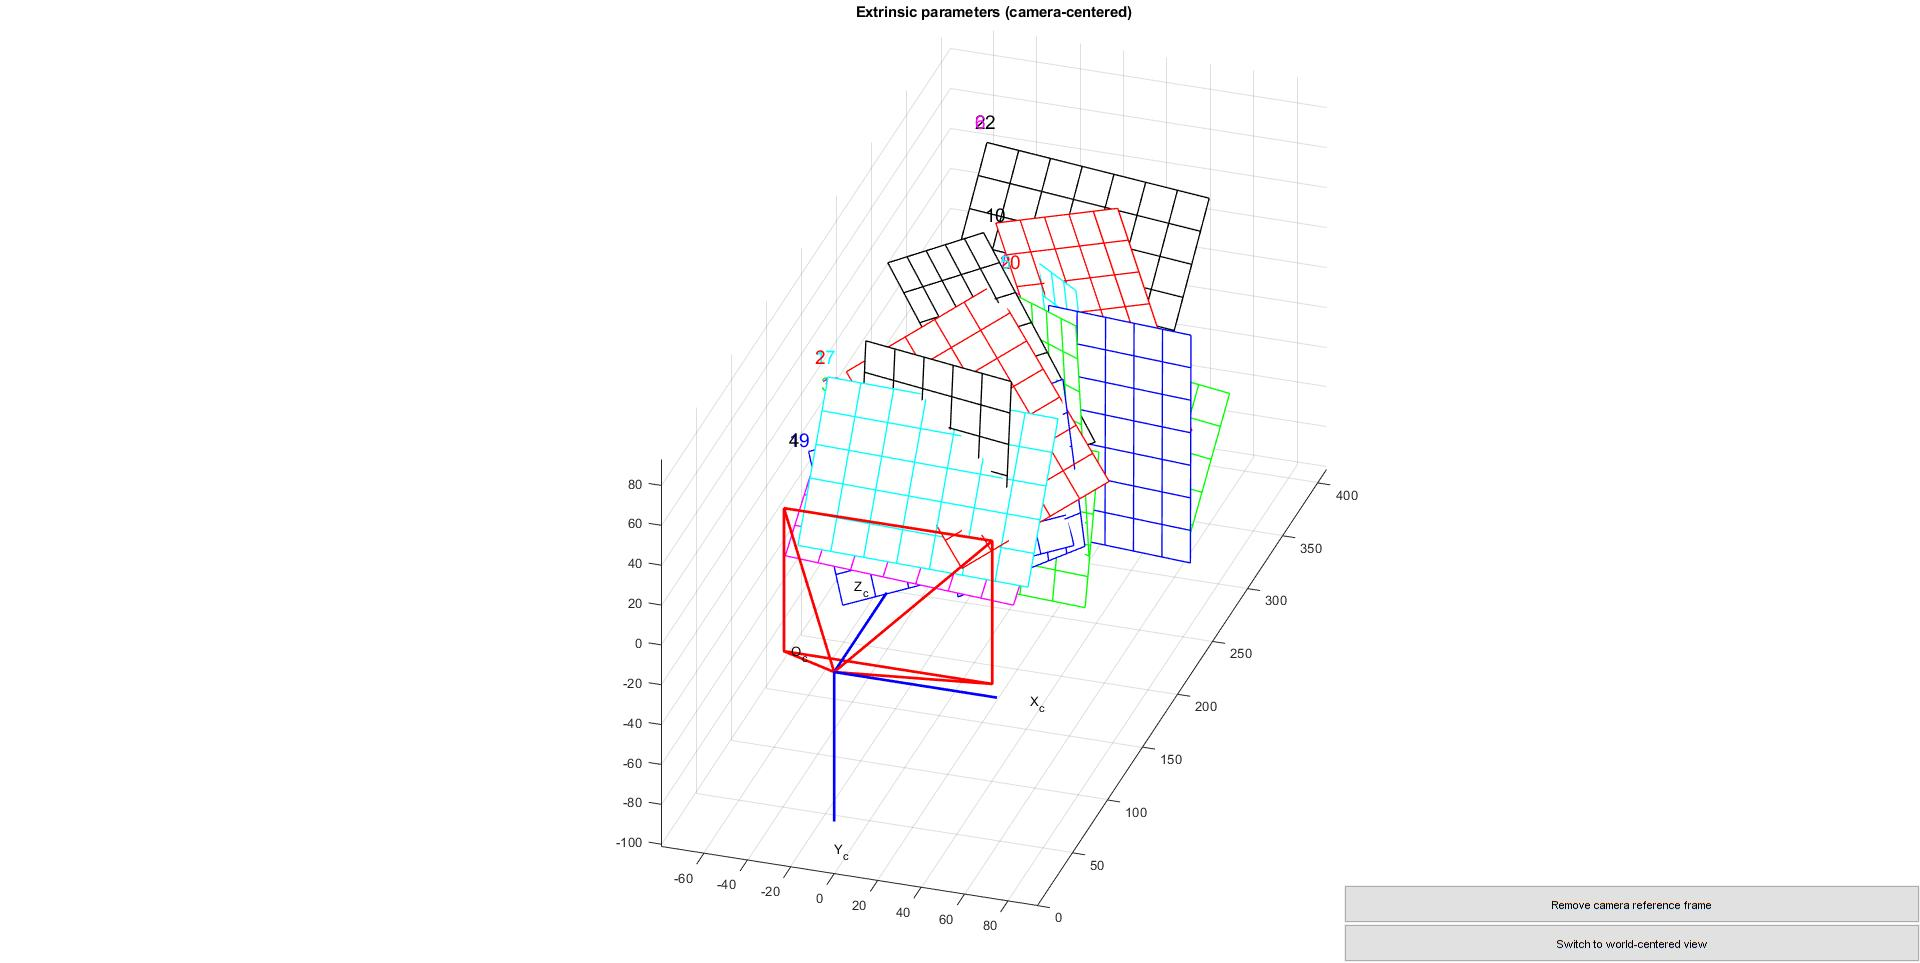
\includegraphics[width=0.5\textwidth]{images/camera_views.jpg}
    \caption{Camera Views.}
    \label{fig:fig1_cal}
    \end{figure}
    
    \begin{figure}[H]
    \centering
    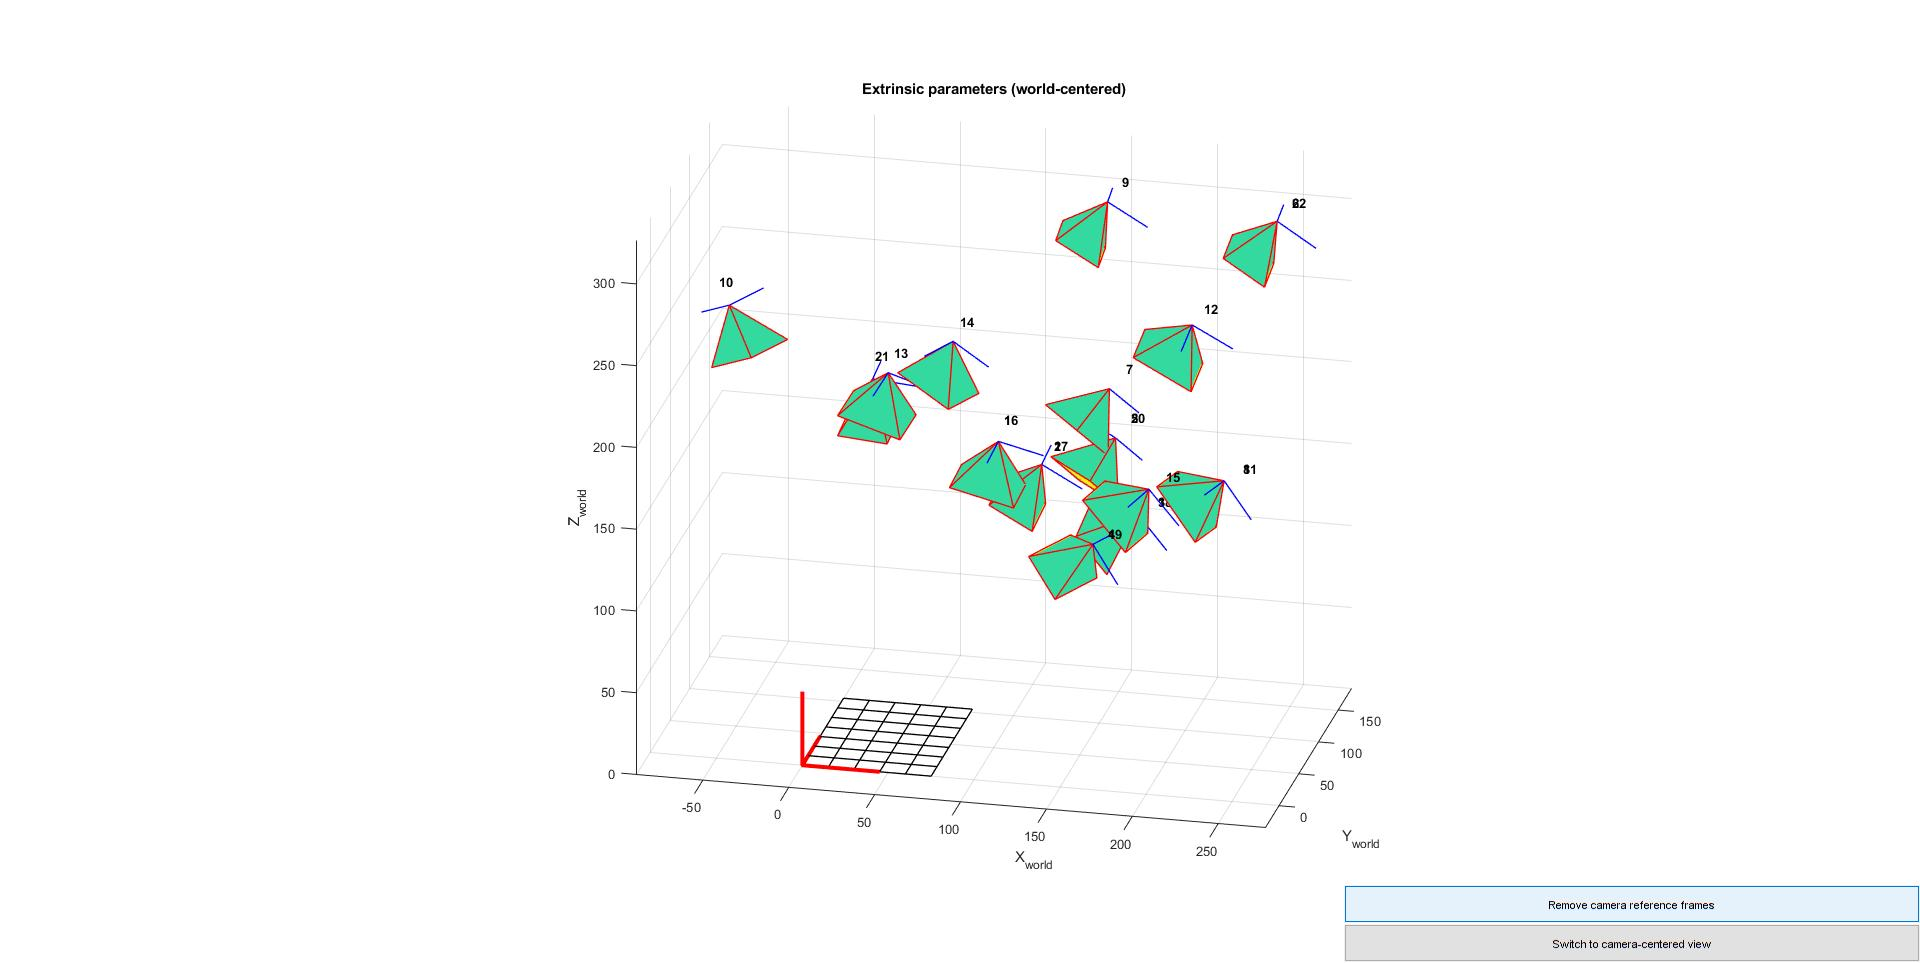
\includegraphics[width=0.5\textwidth]{images/3dcv_cameras.jpg}
    \caption{View of the plane.}
    \label{fig:fig2_cal}
    \end{figure}
    In this section we use the calib tool to observe the different views of images with a camera as a reference in Fig. \ref{fig:fig1_cal}, in the same way in Fig. \ref{fig:fig2_cal} the same fact is observed but with a fixed image.

    \item \textbf{Investigate the re projection error of the camera calibration.}\\
The re projection error can depend on a number of factors such as the type of camera calibration algorithm used, the accuracy of the input data, and the precision of the output coordinates. Generally, however, any errors in the camera calibration will result in a discrepancy between the actual position of
    %%%%Error of the calibariaon
    \begin{figure}[H]
        \centering
        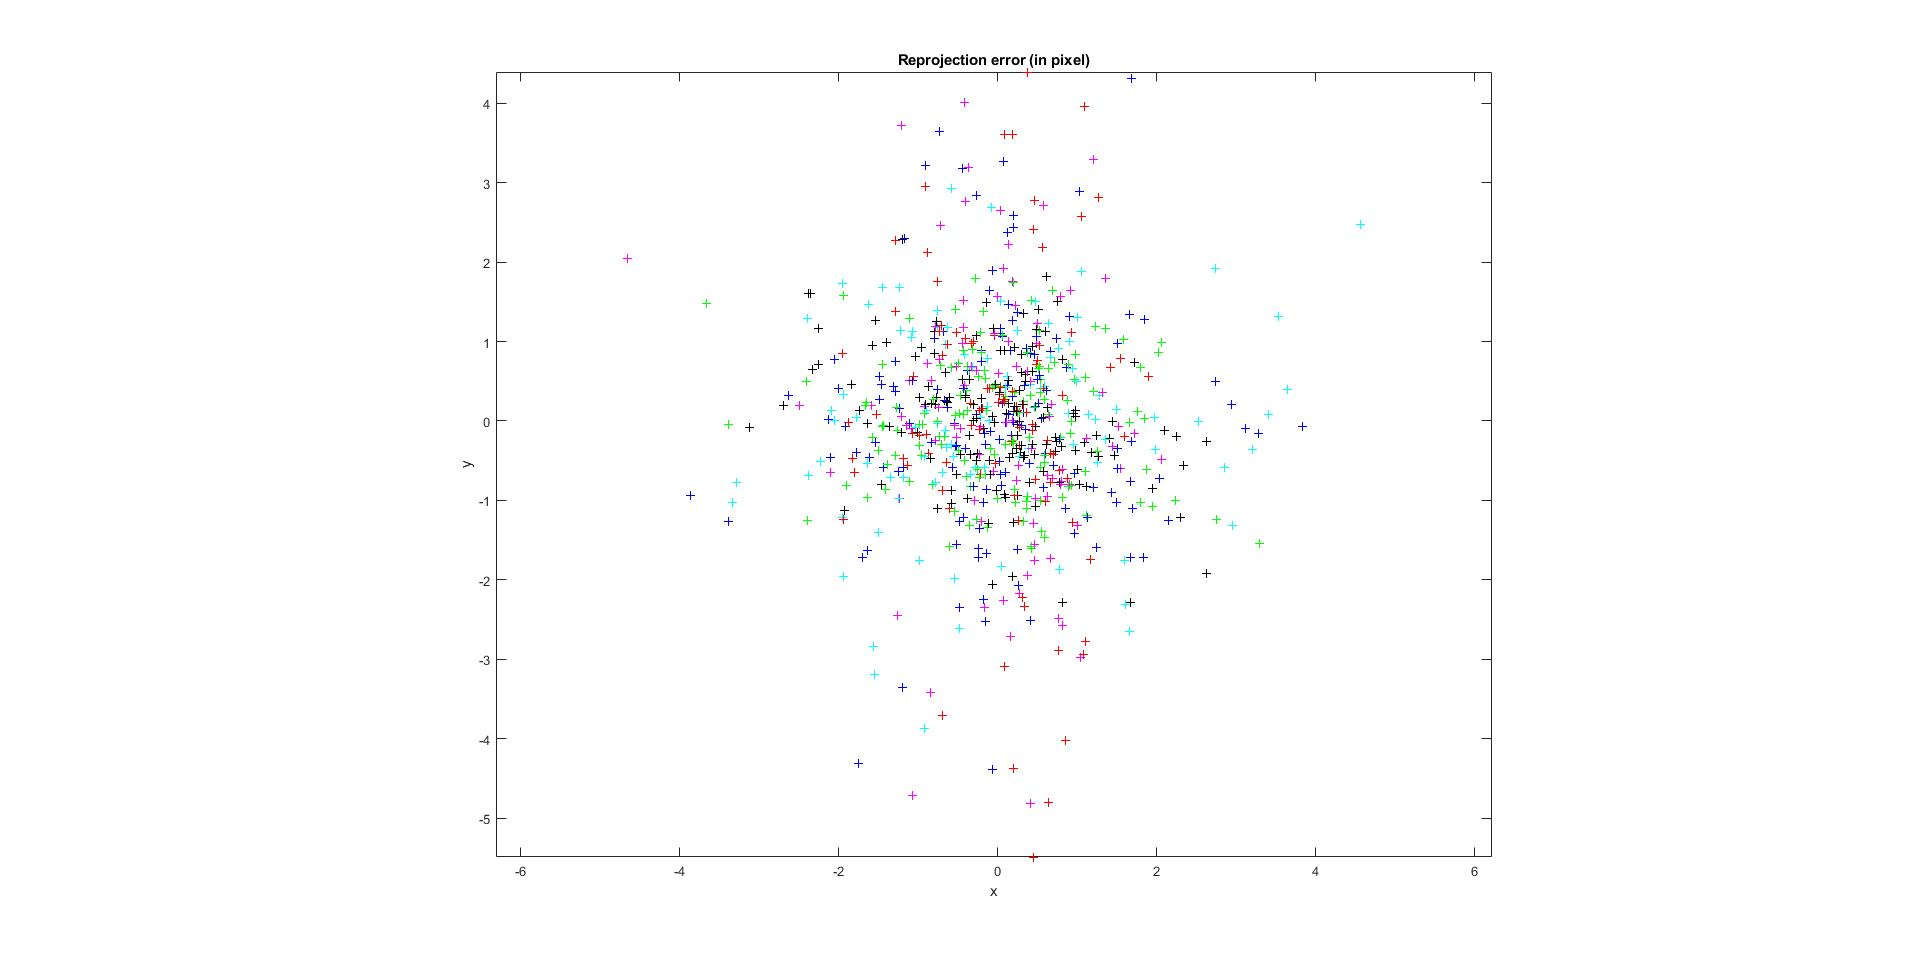
\includegraphics[width=0.5\textwidth]{images/error1.jpg}
        \caption{Calibration error of the cameras.}
        \label{fig:fig2_cal}
    \end{figure}
    
    In this way, in Fig. \ref{fig:fig2_cal}, it can be seen how the error is distributed along a central point that is (0,0), the propagation of the error becomes not considerable, taking into account the resolution of the images taken that \textit{(3024x 4024)}, in the future we could proceed to perform the compression of this image using different kernels if necessary.
    \item \textbf{Save camera intrinsic parameter results for reuse during the last lab.}
    

%%% Parameter of calibration
\begin{figure}[H]
    \centering
    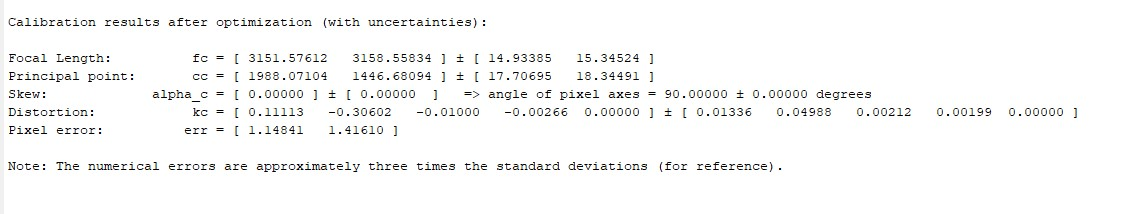
\includegraphics[width=0.5\textwidth]{images/parameters_Calib.jpg}
    \caption{Parameter of calibration.}
    \label{fig:fig3_cal}
\end{figure}



\begin{figure}[H]
     \centering
     \begin{subfigure}[b]{0.3\textwidth}
         \centering
         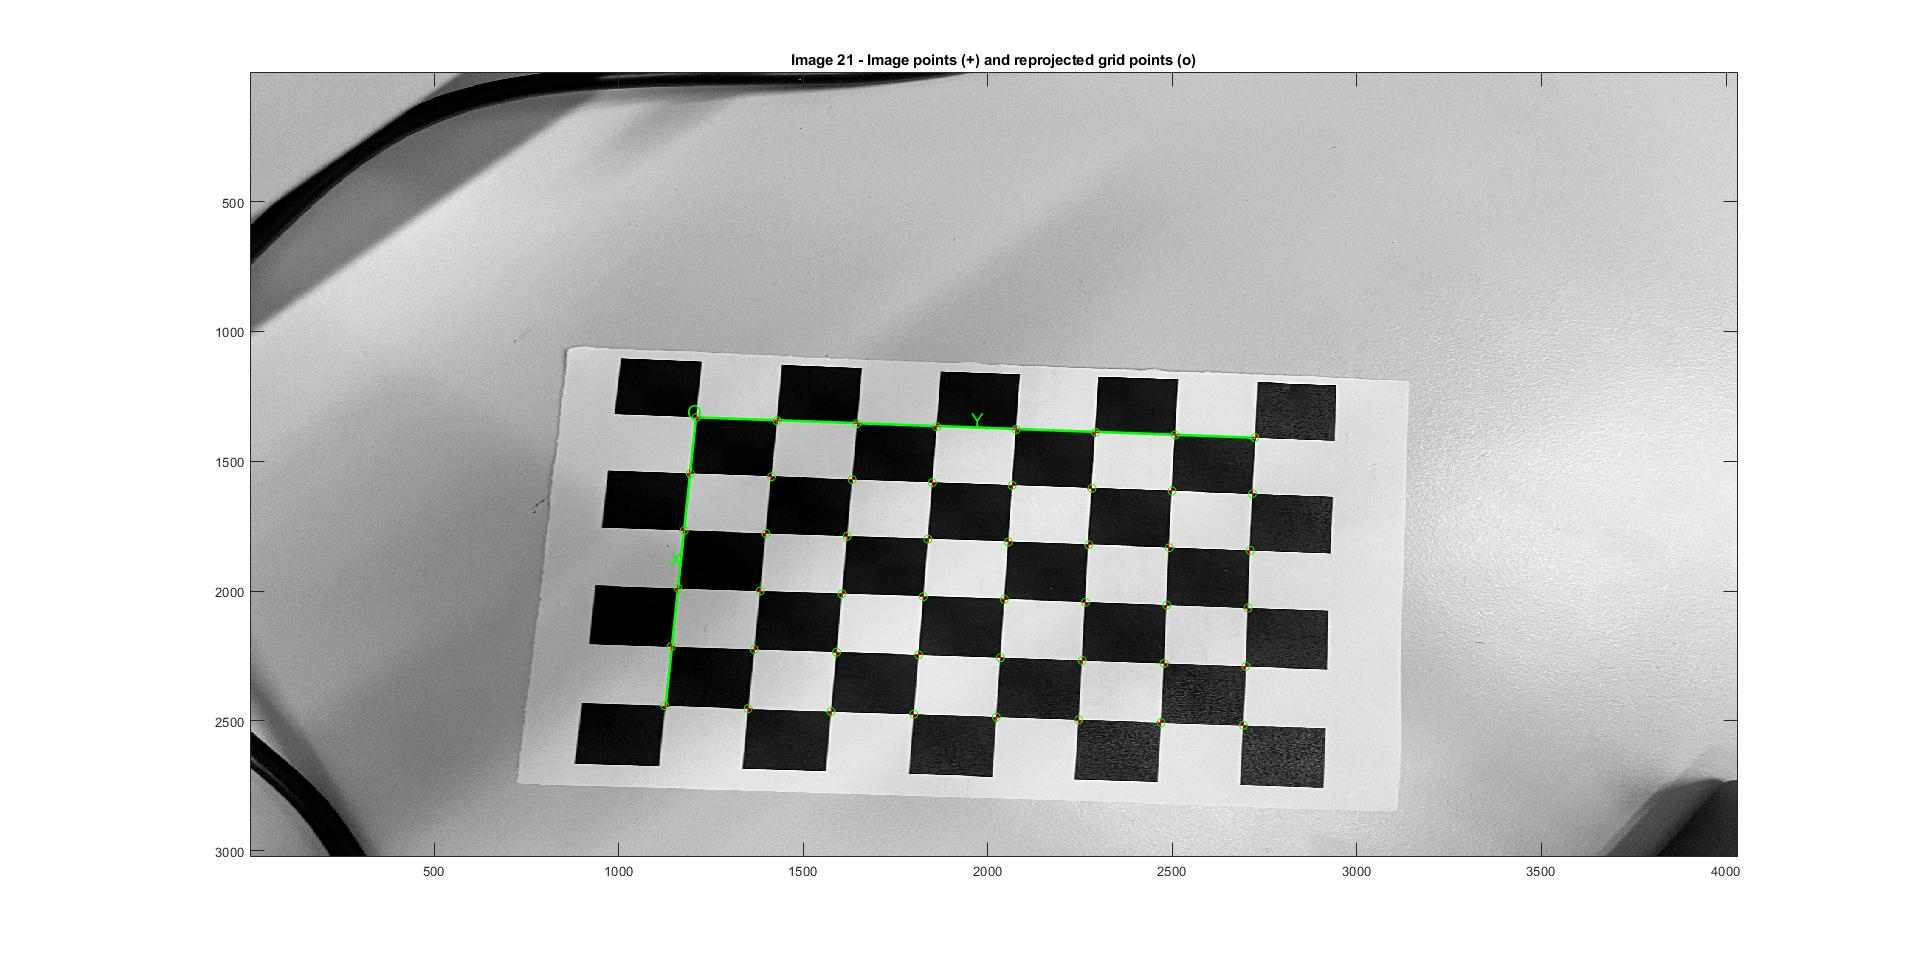
\includegraphics[width=\textwidth]{images/prj1.jpg}
         \caption{Projection 1}
         \label{fig:fig31_cal}
     \end{subfigure}
     \hfill
     \begin{subfigure}[b]{0.3\textwidth}
         \centering
         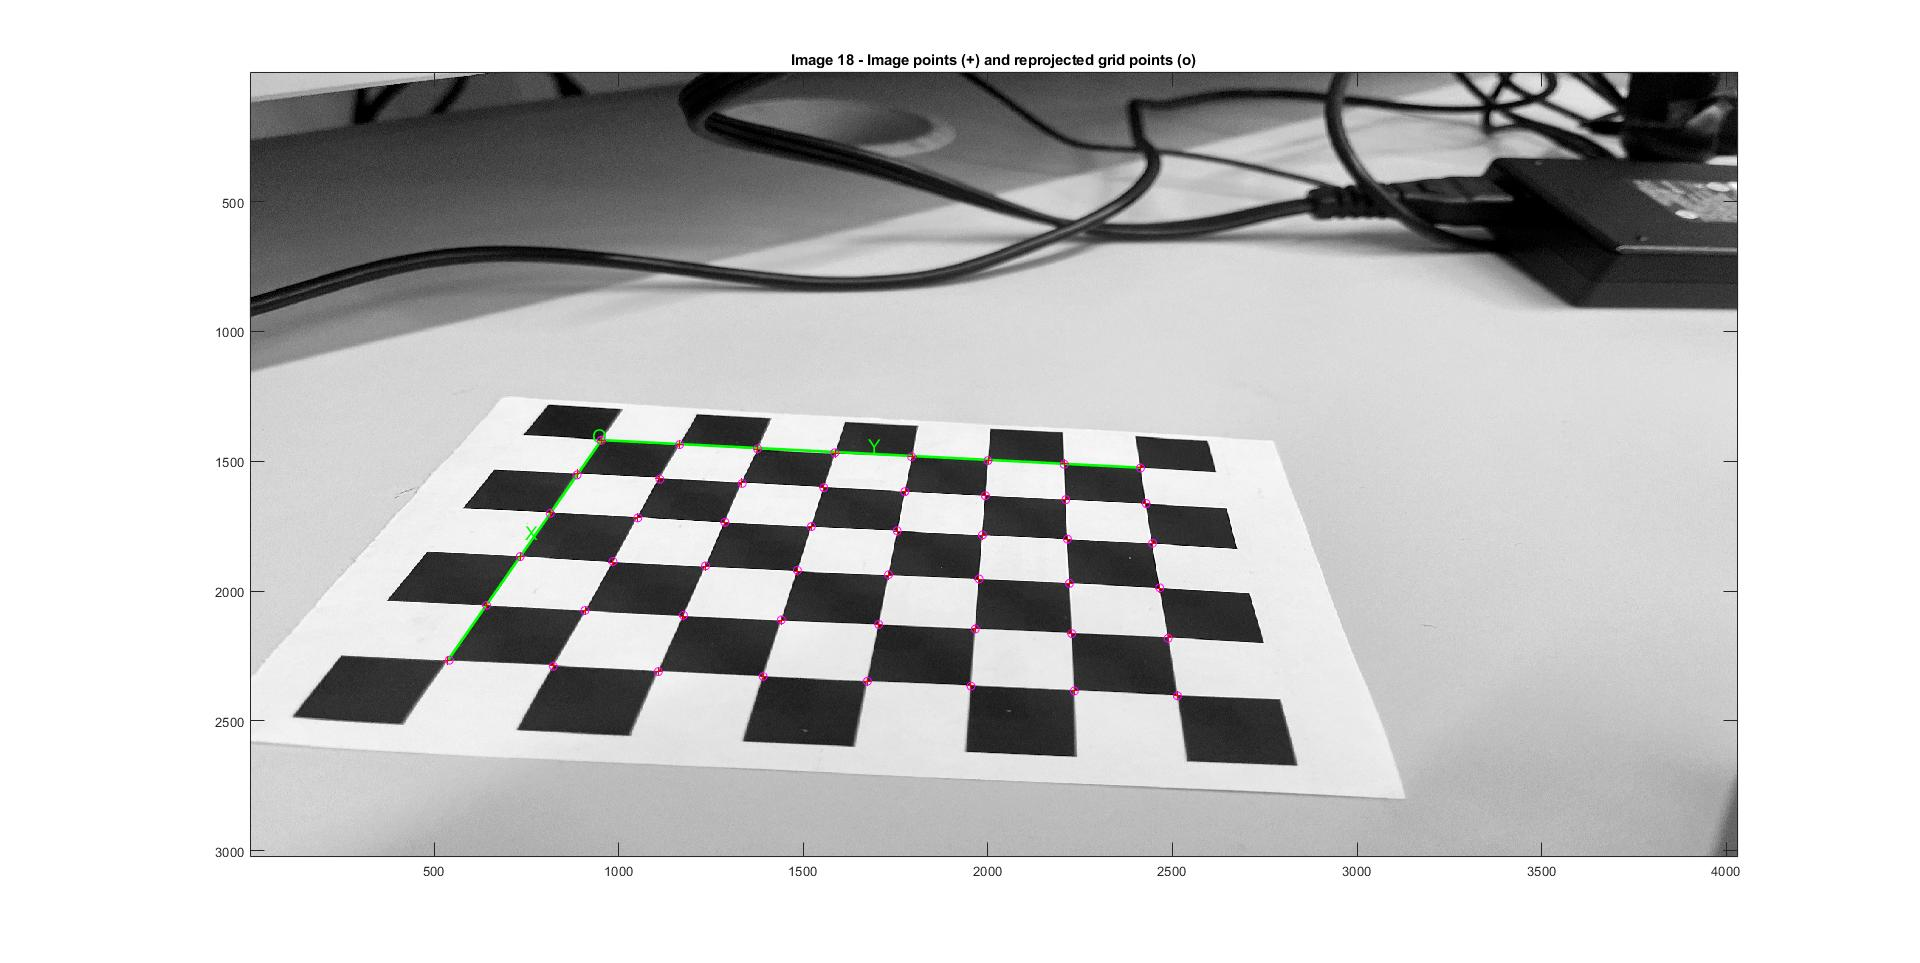
\includegraphics[width=\textwidth]{images/prj2.jpg}
         \caption{Projection 2}
         \label{fig:fig32_cal}
     \end{subfigure}
     \hfill
     \begin{subfigure}[b]{0.3\textwidth}
         \centering
         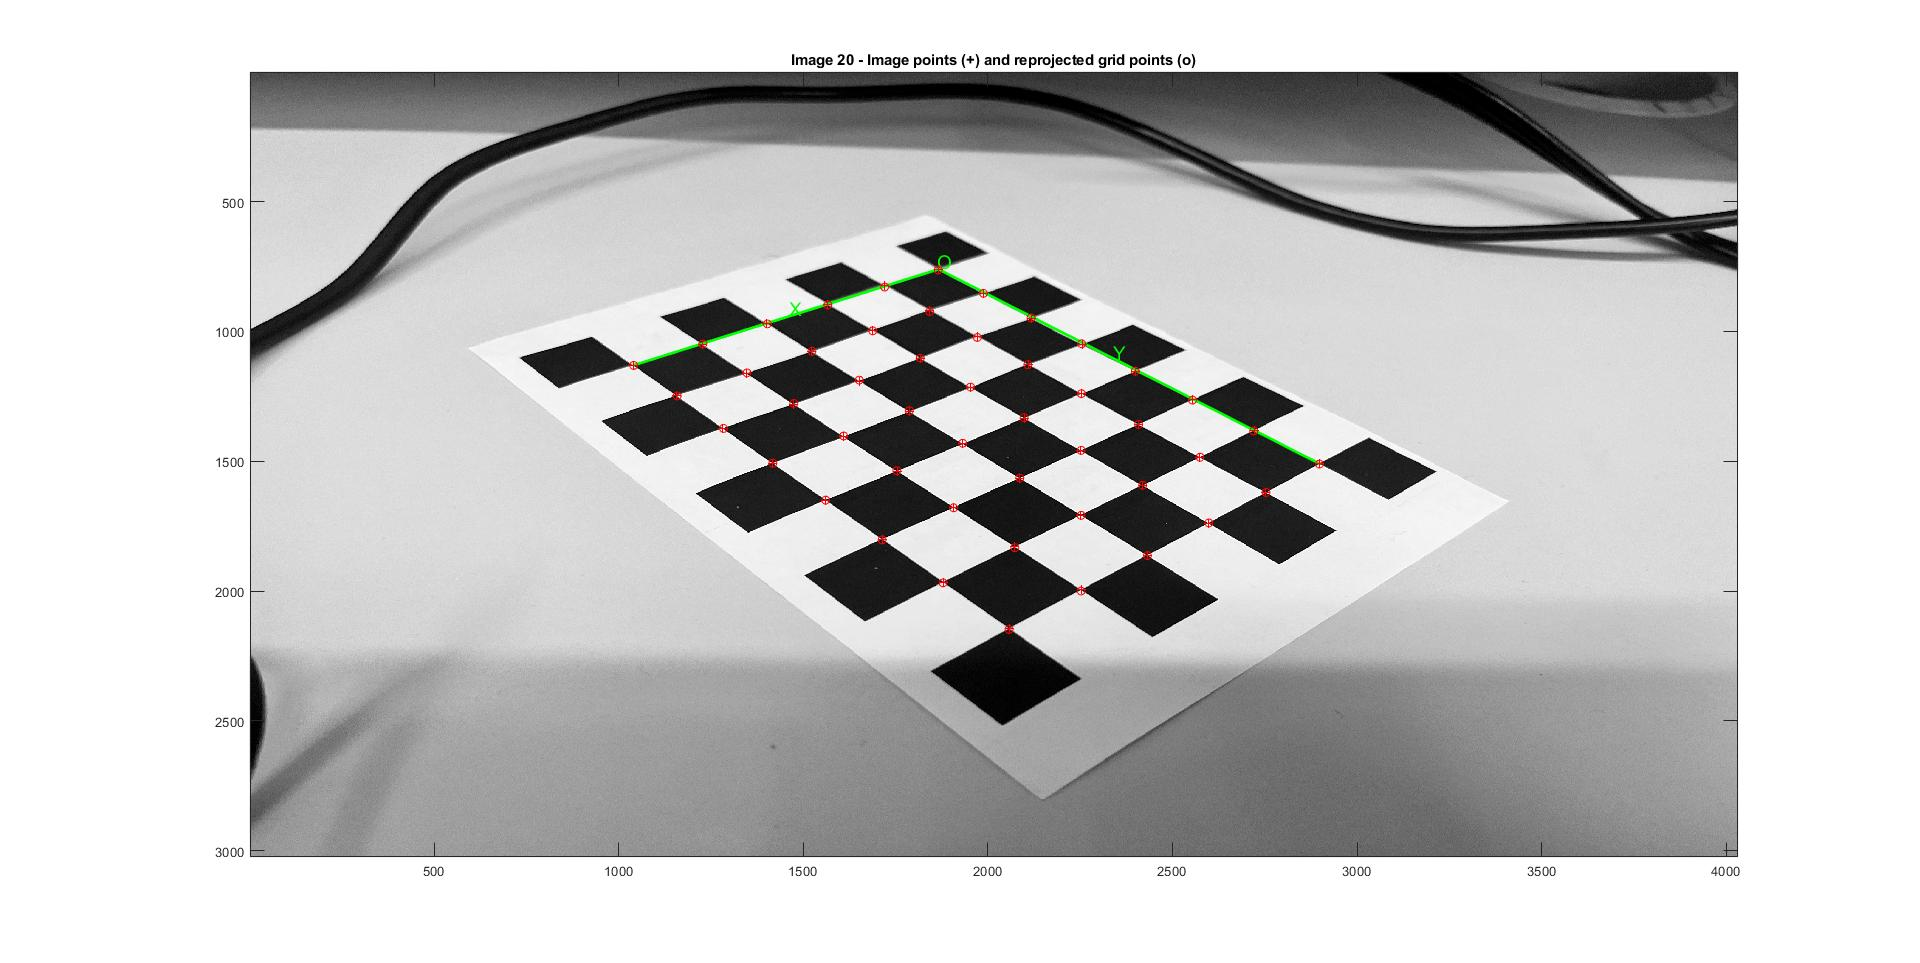
\includegraphics[width=\textwidth]{images/prj3.jpg}
         \caption{Projection 3}
         \label{fig:fig33_cal}
     \end{subfigure}
     \hfill
 
        \caption{Projections of the model generated over the points}
        \label{fig:steps}
\end{figure}

To finish this section, Fig. \ref{fig:fig3_cal} shows the intrinsic parameters of the camera, found for an iPhone 13. This matrix is very useful both for future work and for the tp3, since I tried to find the intrinsic parameters of the camera. of an iPhone and it becomes a restricted data, on the other hand the parameters of the matrix, come to have credibility, because it was compared with parameters of other cameras on the internet, obtaining parameters in similar proportions.\\
It is also observed in Figs. \ref{fig:fig31_cal}, \ref{fig:fig32_cal} and \ref{fig:fig33_cal} the projection of the camera model on test samples, in such a way as to guarantee its validity in a redundant way.
    
\end{enumerate}




%%%%%%%%%%%%






\chapter{Session 2}
The implementation of this section is available in the attached repository at\footnote{\href{https://github.com/GroverAruquipa/3D_Computer_m2}{$https://github.com/GroverAruquipa/3D_Computer_m2$}}.

For this session we try to answer the necessary questions, although not all of them are answered, it is because two questions are the same as one due to the implementation in the code.\\

Homography is important in 3D computer vision because it is a technique that can be used to calculate the transformation between two or more 3D coordinate systems. This can be useful for tasks such as registration (aligning two or more 3D coordinate systems), tracking, and scene reconstruction.

\begin{enumerate}
    \item \textbf{How many matching points should be selected? Why ?}
    According with the equatiosn it is necessary 4 points, in holography, 
There is no definitive answer to this question as it depends on the specific application and the desired level of accuracy. In general, more points should be selected for a more accurate homography..

    
    \item \textbf{Calculate the coefficients $\alpha$, $\beta$, $u$ and $v$ of the matrix K defined in equation 6.}
    In this case, the intrinsic ipatameters of the camera are found from the previous calibration, which will later be multiplied by a transformation matrix based on rotation and translation in section 3, so these parameters are given by:
    \begin{equation}
    K=
        \begin{bmatrix}
3151 & 0 & 1988\\
0 & 0 & 1444\\
0 & 0 & 1
\end{bmatrix}
    \end{equation}
    \item \textbf{Implement the normalize function pts which takes as input the image and the points and gives output normalized points in space $[-1,1 ] x [-1,1 ]$}\\
The normalization function is given from the use of the extreme points of the image and their proper correlation. The following code section shows the correct normalization for this case:
\begin{lstlisting}
% normalization of this points to have points in [-1,1]*[-1,1] as 
% pix1 = K1*ptsNorm1 and pix2 = K1*ptsNorm2
function [ptsNorm, K] = normalise_pts(pts, img) %% pts and img
    alpha=490/2;
    beta=700/2;
    u=490/2;
    v=700/2;
    K=[alpha 0 u; 0 beta v; 0 0 1];
    for i=1:size(pts,1)
        ptsNorm(i,:)=(K\[pts(i,:),1]')';
    end
end 
\end{lstlisting}

    \item \textbf{What mathematical calculation should be implemented in the homography calculation function?}\\
    In order to find the homography matrix, its unnecessary to find the Kronecker product between the homography points which will give us a a matrix, where is necessary to find the pseudo inverse using \textit{Singular Value Decomposition}, an take the variable \textit{v} for the reshaping, the principal equation to solve is defined as:\\
    \begin{equation}
        Ah=0
    \end{equation}
    
    Where A is defined as the Kronecker product between the hmography points mad $h$ is defined as :\\
    \begin{equation}
        h=[h_1 \, h_2 \, h_3 \, h_4 \, h_5 \, h_6 \, h_7 \, h_8]^T
    \end{equation}
    
    \item \textbf{Implement the homography calculation function (ptsNorm1, ptsNorm2, K1, K2) which takes into
inputs two sets of matching normalized points and the normalization matrix and returns the matrix
associated homography}
For this section, two functions were implemented that get the same result, both are presented as a solution for this problem.
This first function shows the Kronecker product developed for 4 points.
\begin{lstlisting}
    function H=homography(x1,y1,x2,y2,x3,y3,x4,y4 , xp1,yp1,xp2,yp2,xp3,yp3,xp4,yp4) %
    % HOMOGRAPHY  Apply homography to points    
    A=[
        -x1  -y1  -1   0    0    0   x1*xp1   y1*xp1   xp1;
         0    0    0 -x1   -y1  -1   x1*yp1   y1*yp1   yp1;
        -x2  -y2  -1   0    0    0   x2*xp2   y2*xp2   xp2;
         0    0    0 -x2   -y2  -1   x2*yp2   y2*yp2   yp2;
        -x3  -y3  -1   0    0    0   x3*xp3   y3*xp3   xp3;
         0    0    0 -x3   -y3  -1   x3*yp3   y3*yp3   yp3;
        -x4  -y4   -1  0    0    0   x4*xp4   y4*xp4   xp4;
         0    0    0  -x4  -y4  -1   x4*yp4   y4*yp4   yp4];       
        [~,~,V] = svd(A);
        H=V(:,end);
        % normalizing homography matrix
        H = reshape(H,3,3);
        for i=1:3
            for j=1:3
                H(i,j)=H(i,j)/H(3,3);
            end
        end
    
end
\end{lstlisting}
Unlike the previous one, the following function shows a general function for n points if necessary:
\begin{lstlisting}
    % homography 2H1 from img2 to img1
function [H] = calcul_homographie(ptsNorm1, ptsNorm2, K1, K2)
    H = zeros (3,3);
    A = zeros (3*size(ptsNorm1,1),9);
    
    % A = [p2]^ x tp1
    for i=1:size(ptsNorm1,1)
        A(3*i-2,:) = [0 0 0 -ptsNorm2(i,1) -ptsNorm2(i,2) -1 ptsNorm1(i,2)*ptsNorm2(i,1) ptsNorm1(i,2)*ptsNorm2(i,2) ptsNorm1(i,2)];
        A(3*i-1,:) = [ptsNorm2(i,1) ptsNorm2(i,2) 1 0 0 0 -ptsNorm1(i,1)*ptsNorm2(i,1) -ptsNorm1(i,1)*ptsNorm2(i,2) -ptsNorm1(i,1)];
        A(3*i,:) = [0 0 0 0 0 0 ptsNorm2(i,1) ptsNorm2(i,2) 1]; % 3eme ligne de A
    end
    % applying svd
    [u, s, v] = svd(A);
    h = v(:,end);
	Hbis = reshape(h,3,3)';
    H = inv(K2) * Hbis * K1;
    H = H/H(3,3);% normalisation0
  
end
\end{lstlisting}

    \item \textbf{How to check the validity of the computed homography matrix?}\\
    To verify the validity, it is necessary to multiply the holography from 1 to 2 and in the same way from 2 to 1, in such a way as to carry out the multiplication and obtain an identity matrix, as shown in the attached codes.
    For this case the matrix was obtained:
    \begin{equation}
    M=
        \begin{bmatrix}
1.1616 & 0 & 0\\
0 & 1.1616 & 0 \\
0 & 0 & 1.1616
\end{bmatrix}
    \end{equation}
    Observing the previous matrix it can be indicated that the calculation of the homography is done correctly.
    \item \textbf{Implement this algorithm in the function mosaic 2in1(img1,img2, H1 2). Display the result with I2 pasted in I1, then with I1 pasted in I2. Although this algorithm performs well, it has two major flaws, one of them is (obviously) the time quite substantial calculation.}

\begin{lstlisting}
    function [img] = mosaic_2in1(img1, img2,pix1,pix2, H)
% Calculate the transformation of the 4 corners of the image img1 in the image img2
% and find the min and max values of the coordinates
% to define the size of the mosaic image
% img1: image 1
% img2: image 2
% nbPix: number of pixels to add to the size of the mosaic image
% H: homography matrix
% img: mosaic image
%pix1 is the pixel matched in img1
%pix2 is the pixel matched in img2
% Calculate the transformation of the 4 corners of the image img1 in the image img2
nbPix=3;
corners = [1 1; size(img1,2) 1; size(img1,2) size(img1,1); 1 size(img1,1)];
corners = [corners ones(4,1)]';
corners = H*corners;
corners = corners./repmat(corners(3,:),3,1);
corners = corners(1:2,:)'
%find the size of the mosaic image
minX = min(corners(:,1));
maxX = max(corners(:,1));
minY = min(corners(:,2));
maxY = max(corners(:,2));
%round 
minX = floor(minX);
maxX = floor(maxX);
minY = floor(minY);
maxY = floor(maxY);

% for each pixel of the mosaic image find the corresponding pixel in the image img1 
% and the corresponding pixel in the image img2
% and make the average of the 2 pixels
img = zeros(maxY-minY+nbPix,maxX-minX+nbPix,3);
for i=1:size(img,1)
    for j=1:size(img,2)
        % find the corresponding pixel in the image img1
        p = [j+minX-1 i+minY-1 1]';
        p = inv(H)*p;
        p = p./p(3);
        p = round(p(1:2));
        % if the pixel is inside the image img1
        if p(1)>0 && p(1)<=size(img1,2) && p(2)>0 && p(2)<=size(img1,1)
            % find the corresponding pixel in the image img2
            p2 = [j+minX-1 i+minY-1 1]';
            p2 = p2';
            % if the pixel is inside the image img2
            if p2(1)>0 && p2(1)<=size(img2,2) && p2(2)>0 && p2(2)<=size(img2,1)
                % make the average of the 2 pixels
                img(i,j,:) = (img1(p(2),p(1),:)+img2(p2(2),p2(1),:))/2;
            else
                img(i,j,:) = img1(p(2),p(1),:);
            end
        else
            % find the corresponding pixel in the image img2
            p2 = [j+minX-1 i+minY-1 1]';
            p2 = p2';
            % if the pixel is inside the image img2
            if p2(1)>0 && p2(1)<=size(img2,2) && p2(2)>0 && p2(2)<=size(img2,1)
                img(i,j,:) = img2(p2(2),p2(1),:);
            end
       
    end
end
end
% show the mosaic image
figure;
imshow(uint8(img));

end
\end{lstlisting}
This first algorithm was sought to improve in an intuitive way, firstly the image corners were calculated, in the same way 4 points of each image for the correlation, in this way having the homography matrix for both images previously we proceeded to re-correct the image with a $for$ cycle and fill in the necessary points, previously applying the homography matrix, depending on the progress in classes.

    \item \textbf{What alters the mosaic result, especially when the pasted image is larger than
the original picture?}\\
The mosaic result will be altered if the pasted image is larger than the original picture. The pasted image will be resized to fit the original picture, and some of the edges of the pasted image may be cropped.
    \item \textbf{What is the difference between the two algorithms?}

According to the instructions in the first algorithm, the limits are not prioritized and take into account the total image compared to the second one where a better result is sought, despite this it has a higher latency for the search for pixels, That is why it is advisable to change the size of the image beforehand.

\begin{figure}[H]
    \centering
    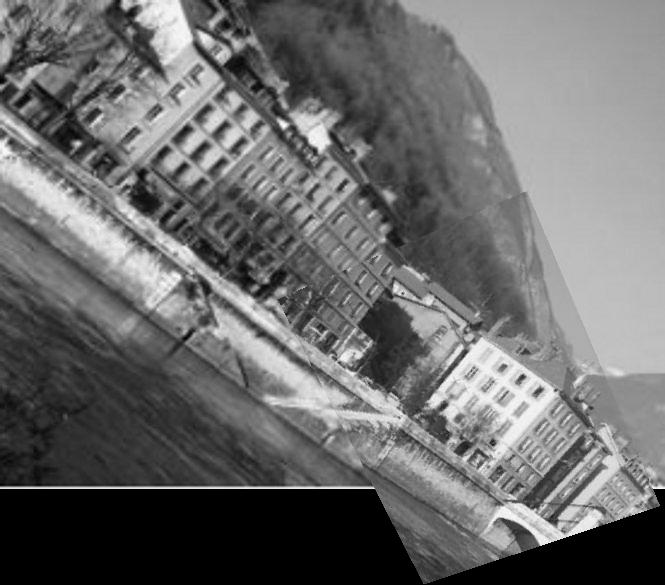
\includegraphics[width=0.5\textwidth]{images/mosaicing05img.jpg}
    \caption{Creation of the mosaic of the image.}
    \label{fig:fig2_mos}
\end{figure}


\item \textbf{Implement this second algorithm in the function mosaic and test it}

\begin{figure}[H]
    \centering
    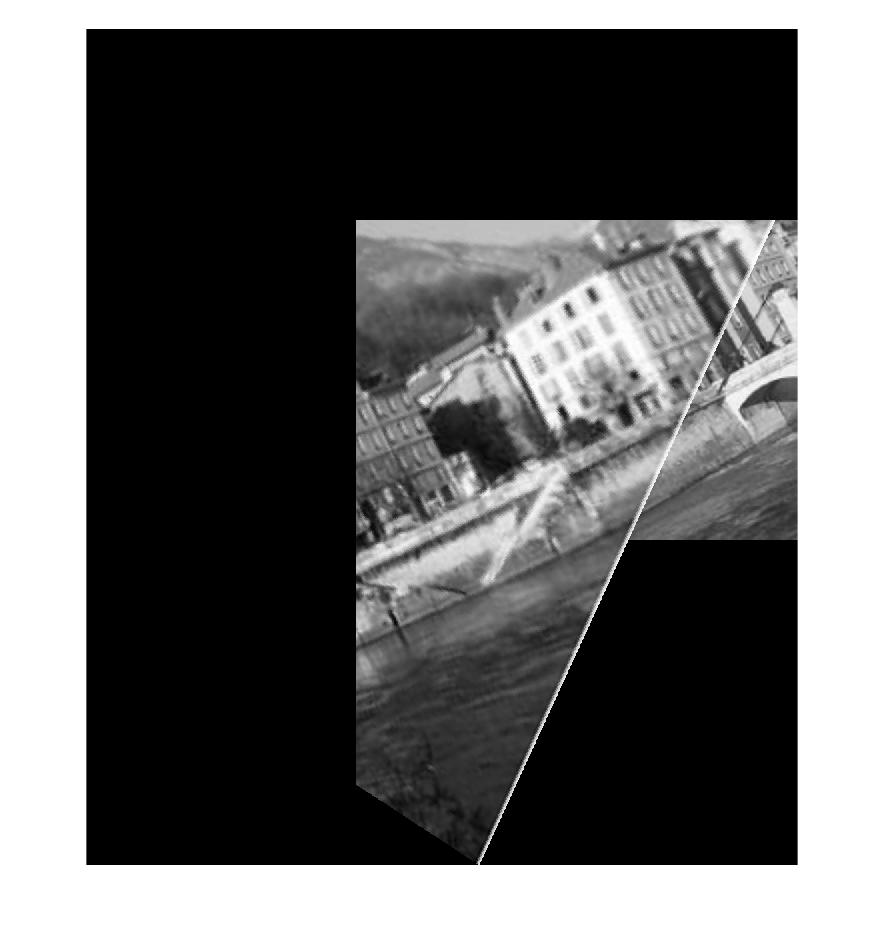
\includegraphics[width=0.5\textwidth]{images/tp_3/mosaic2.jpg}
    \caption{Mosaic of the Image 1.}
    \label{fig:fig1_mosc}
\end{figure}

\item \textbf{Implement the function mosaic bis(img1, img2, H2 1) which uses the algorithm described in the previous section taking as input two images and two sets of matching points and returns the mosaic
of the two pictures.} - \textbf{Augment the mosaic() function so that it returns a color image.}
In this section is it possible to find the answer for two questions.

\begin{lstlisting}
    % Best Method
function [temp] = mosaic_bis(img1, img2, pix1,pix2, H)
    IH=inv(H); % inverse of homography matrix
    trans_points=[1 1 1] * IH;
    x1=trans_points(1,1)/trans_points(1,3); %Normalize the points
    y1=trans_points(1,2)/trans_points(1,3); %Normalize the points
    trans_points=[1,size(img2,1), 1] * IH; %Normalize the points
    x2=trans_points(1,1)/trans_points(1,3);
    y2=trans_points(1,2)/trans_points(1,3);
    
    trans_points=[size(img2,2),1, 1] * IH;
    x3=trans_points(1,1)/trans_points(1,3);
    y3=trans_points(1,2)/trans_points(1,3);
    trans_points=[size(img2,2), size(img2,1), 1] * IH;
    x4=trans_points(1,1)/trans_points(1,3);
    y4=trans_points(1,2)/trans_points(1,3);
    
    corners=[x1 y1;x2 y2;x3 y3;x4 y4;1 1;1 ,size(img1,1);size(img1,2), 1;size(img1,2),size(img1,1)];
    % corners=[x1 y1;x2 y2;x3 y3;x4 y4;1 1;1 ,size(img1,1);size(img1,2), 1;size(img1,2),size(img1,1)];
    MAX_X=0;
    for i=1:8
        if MAX_X<= corners(i,1)      %calcluate the max x wothout using max function
        MAX_X=corners(i,1);
        end
    end

    MAX_Y=0;
    for i=1:8
        if MAX_Y<= corners(i,2)      % calculate the max y without using max function
        MAX_Y=corners(i,2);
        end
    end
    
    
    MIN_X=0;
    for i=1:8
        if MIN_X>= corners(i,1)      % calculate the min x without using min function
        MIN_X=corners(i,1);
        end
    end
 
    MIN_Y=0;
    for i=1:8
        if MIN_Y>= corners(i,2)      % calculate the min y without using min function
        MIN_Y=corners(i,2);
        end
    end
  max_height=round(MAX_Y-MIN_Y);     % maximum height of new image 
    max_width=round(MAX_X-MIN_X);      % maximum width of new image
    x_offset=round(abs(MIN_X));        % x offset for new image
    y_offset=round(abs(MIN_Y));        % y offset for new image
   
    % Create new image with the maxium size
    temp = zeros(max_height,max_width); % create a new image with zeros
    temp=im2double(temp); % convert to double for intensity values
    %%
    % Prepare the image for the transformation by copying the intensity values of the first image
    for i=1:size(img1,1)
        for j=1:size(img1,2)
             temp(i+y_offset,j+x_offset,1)=img1(i,j,1);  % copy intensity values of image 1
            temp(i+y_offset,j+x_offset,2)=img1(i,j,2); % copy intensity values of image 1
            temp(i+y_offset,j+x_offset,3)=img1(i,j,3); % copy intensity values of image 1
           
        end
     end
    figure, imshow(temp);
    
    %% Each pixel in the new image is transformed to the original image
    
    for i=1:size(temp,1)
        for j=1:size(temp,2)
            % projected points after applying homography
            projected_point= [j, i, 1]*H; % apply homography to each pixel in the new image
    a1=projected_point(1,1)/projected_point(1,3);  % points in image 2
    b1=projected_point(1,2)/projected_point(1,3);
    a1=round(a1); % rounding values
    b1=round(b1);
    if(a1>=1 && b1>=1 && a1<=size(img2,2) && b1<=size(img2,1))
        temp(i+y_offset,j+x_offset,1)=img2(b1,a1,1);    %red channel
         temp(i+y_offset,j+x_offset,2)=img2(b1,a1,2);   % green channel
          temp(i+y_offset,j+x_offset,3)=img2(b1,a1,3);  % blue channel
    end
        
        end
    end
    figure(); imshow(temp); % display the final image
    
end
\end{lstlisting}
   For this second algorithm, the suggestions shown in the instructions were followed, and in the same way, in order to obtain a time-optimized homography, the calculation was carried out trying to evade the internal functions of Matlab that require a long time, in the first part. What I tried to do is perform the normalization, calculate the corners, m the maximum and t minimum. In this way, we proceeded to prepare the image for the copy of the intensity of the pixels, in order to go through the final image and apply the projection in the second Image, obtaining as a result 1H2 Fig. \ref{fig:fig2_mos}. and for 2H1 pa Fig \ref{fig:fig1_mos}.

     \item \textbf{Test your program on two matching images acquired by you}
     In Fig. \ref{fig:campusP}. The results for the homography are presented with a photograph taken from the university campus, looking for a rectangular structure for the calculation of the homography, in Fig. \ref{fig:campusP}, the selected points are observed in both images and in Fig. \ref{fig:fig1_campus2}, the correct operation performed is observable.
\begin{figure}[H]
     \centering
     \begin{subfigure}[b]{0.9\textwidth}
         \centering
         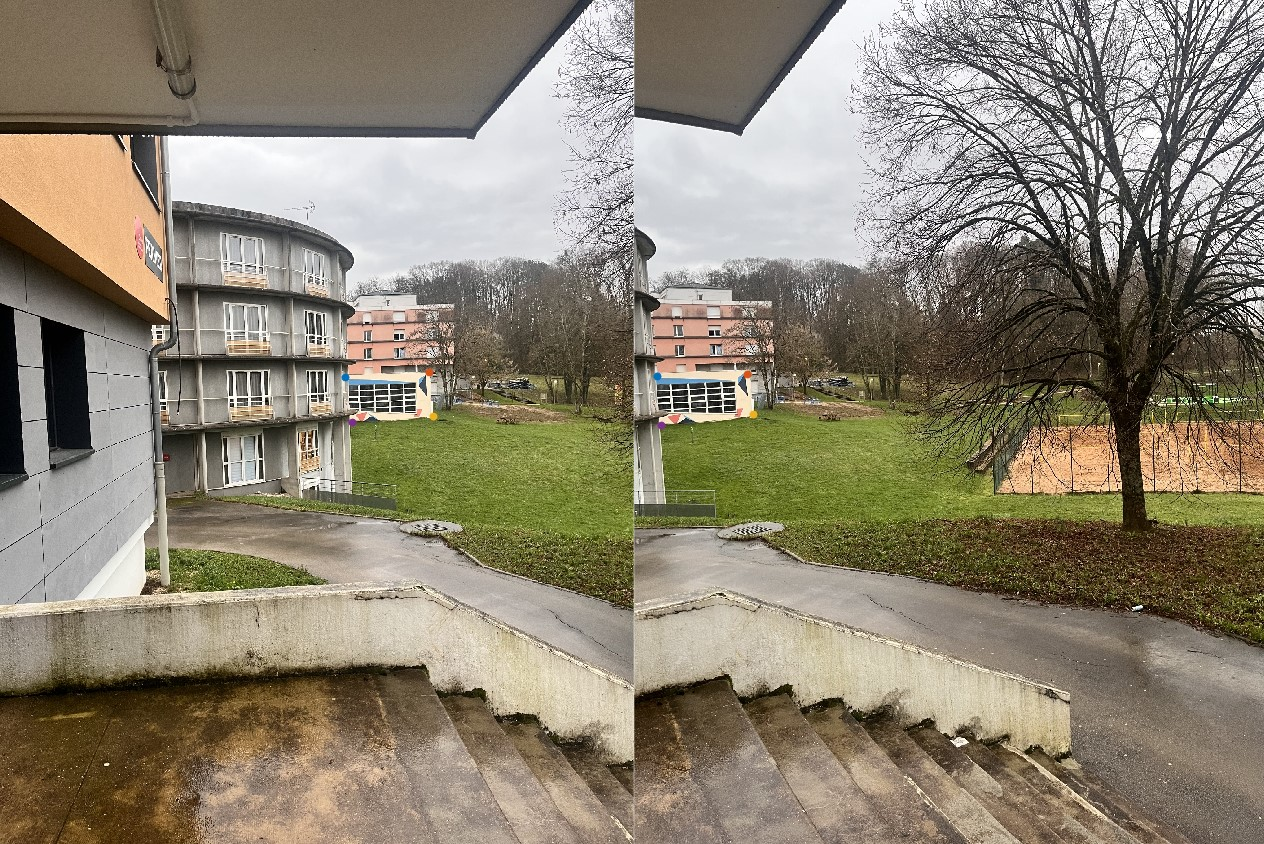
\includegraphics[width=0.8\textwidth]{images/tp_2/panoramic points.jpg}
    \caption{Two images of the campus.}
    \label{fig:fig1campus1}
     \end{subfigure}
     \hfill
     \begin{subfigure}[b]{0.9\textwidth}
         \centering
         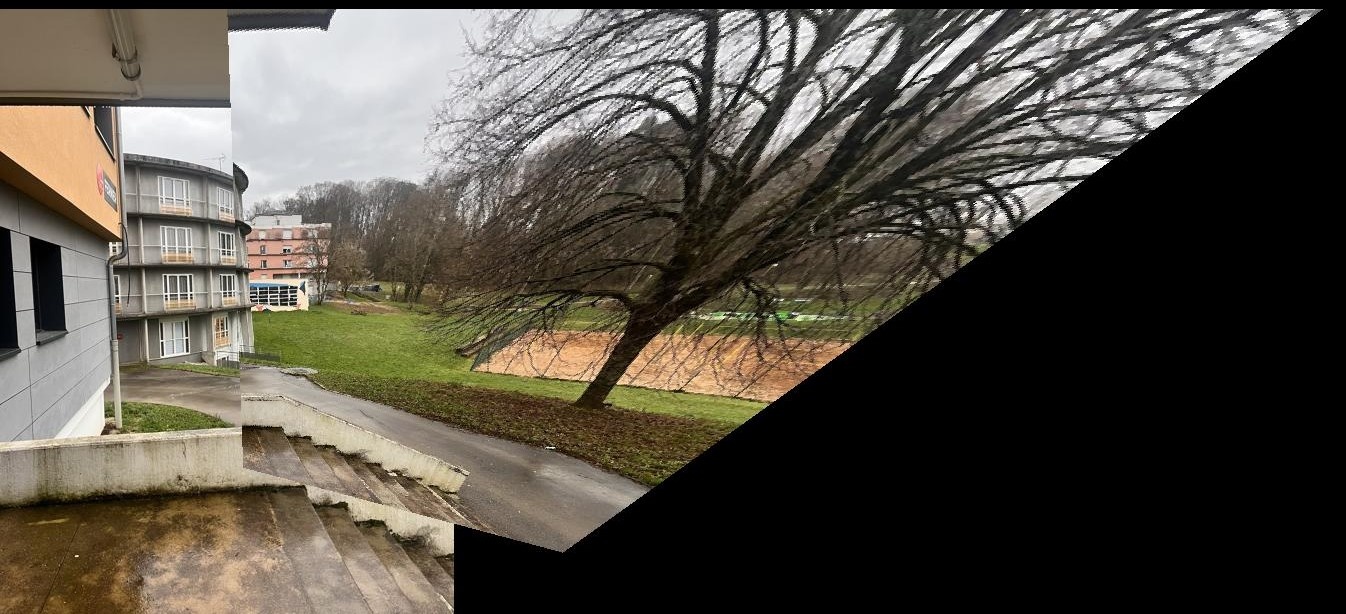
\includegraphics[width=0.8\textwidth]{images/tp_2/panoramic.jpg}
    \caption{Homography of the two images.}
    \label{fig:fig1_campus2}
     \end{subfigure}
     
     \hfill 
        \caption{Homography with images from the campus.}
        \label{fig:campusP}
\end{figure}

\item \textbf{Describe the principle of operation of such an algorithm \textit{RANSAC}.}

The RANSAC algorithm is a method for detecting and removing outliers from a set of data points. It operates by randomly selecting a data point from the set and then checking to see if it is an outlier. If it is, the algorithm removes it from the set. It then repeats this process until no more outliers remain. Finally if we want implement RANSAC, we need have the following considerations:
\subitem{The parameters are estimated from \textit{N} data}
\subitem{The probability of a randomly selected data being part of a good model}
\subitem{It is possible do not  find a good fit}
\item \textbf{Make a rectification of an image chosen by you.}
The rectification of the image was done with extra considerations looking for the correct projection, in Fig. \ref{fig:fig1_rect2} the input image is shown and the rectified image in Fig. \ref{fig:fig1_rect}. This process becomes much simpler due to the use of few resources. computational comparison of homography.
\begin{figure}[H]

     \centering
     \begin{subfigure}[b]{0.9\textwidth}
         \centering
         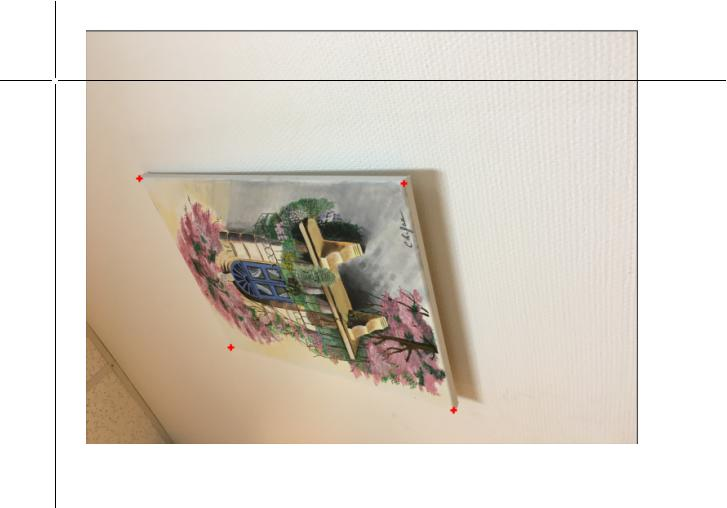
\includegraphics[width=0.5\textwidth]{images/rect0.jpg}
    \caption{Input image.}
    \label{fig:fig1_rect2}
     \end{subfigure}
     \hfill
     \begin{subfigure}[b]{0.9\textwidth}
         \centering
         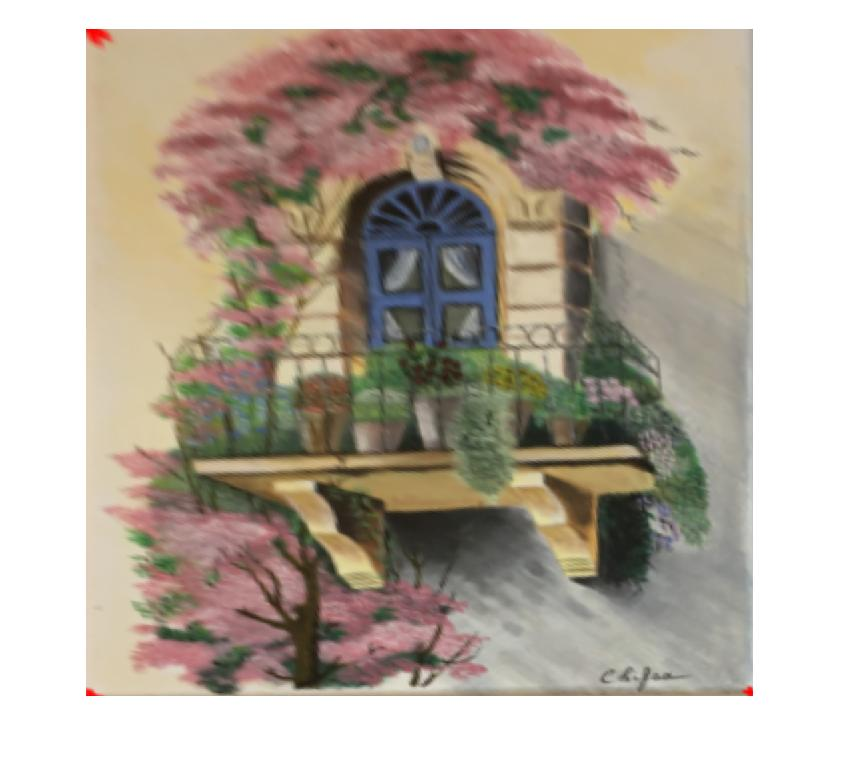
\includegraphics[width=0.5\textwidth]{images/rect1.jpg}
    \caption{Rectification of the Image 3.}
    \label{fig:fig1_rect}
     \end{subfigure}
     
     \hfill 
        \caption{Images Rectified}
        \label{fig:inctotal}
\end{figure}

\item \textbf{Embedding a straight image into another using homography.}

\begin{figure}[H]
     \centering
     \begin{subfigure}[b]{0.3\textwidth}
         \centering
         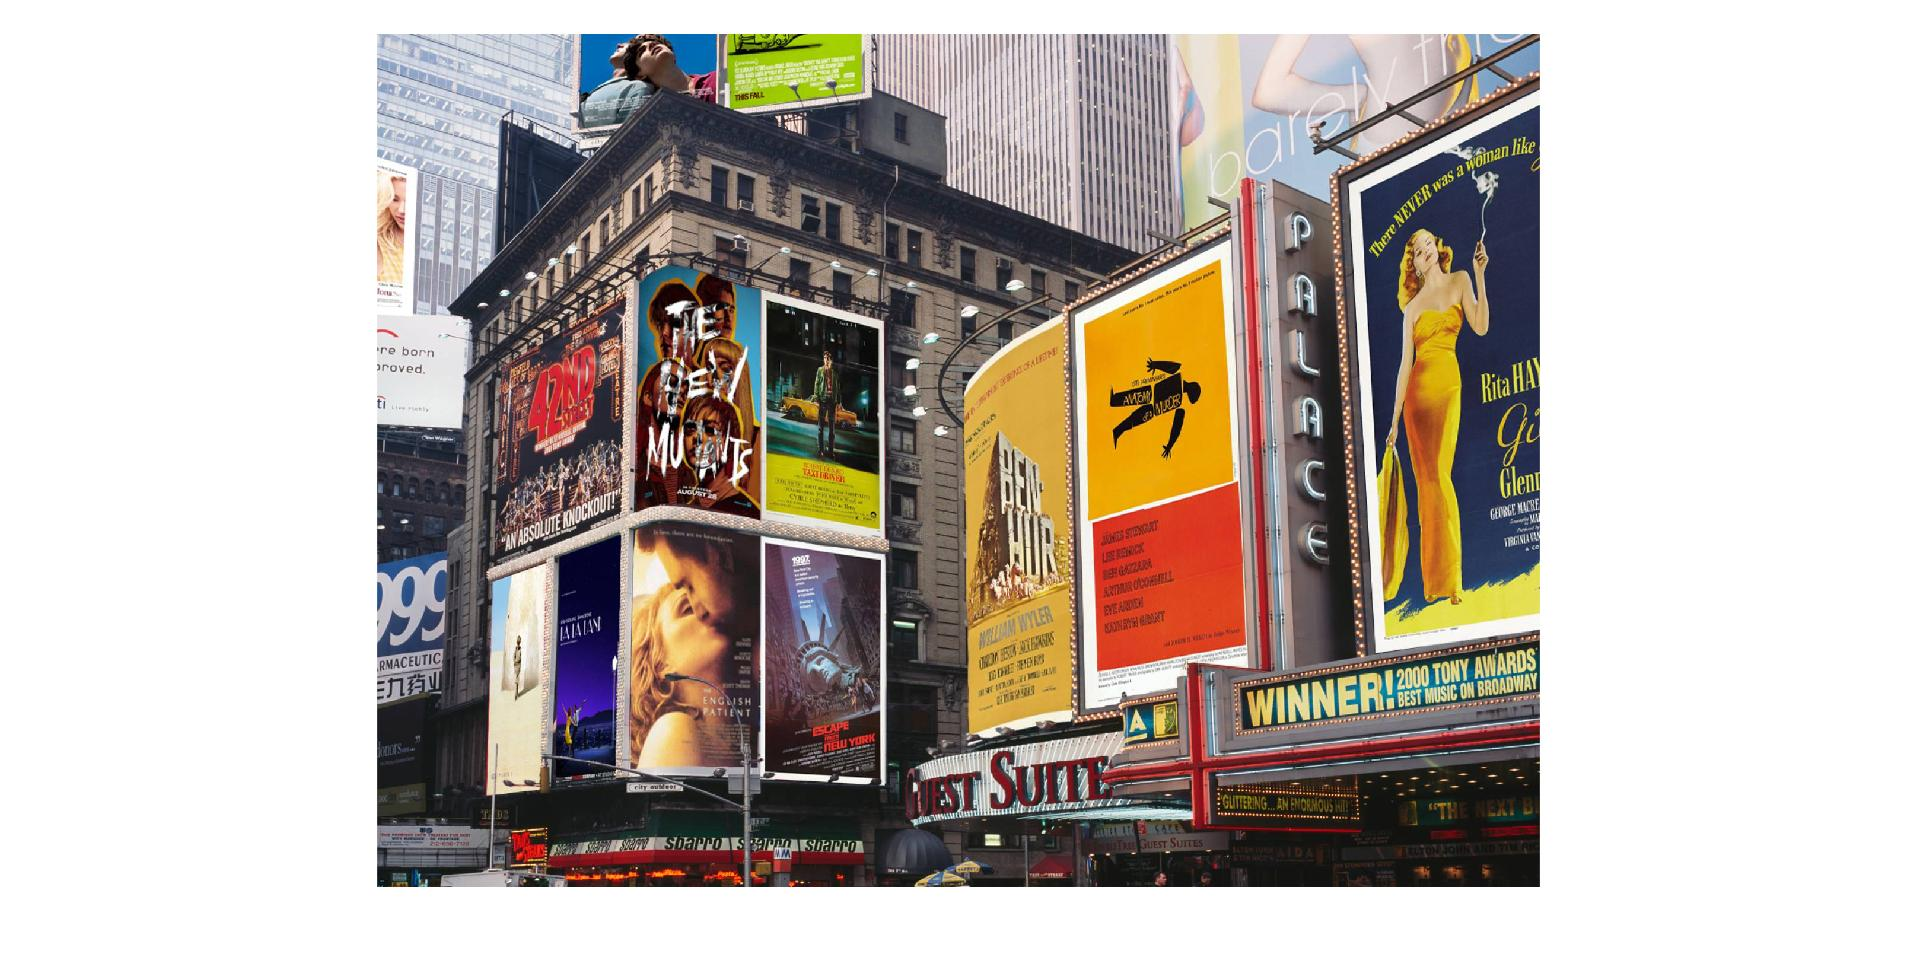
\includegraphics[width=\textwidth]{images/tp_2/incruste1.jpg}
             \caption{Main Image}
         \label{fig:inc1}
     \end{subfigure}
     \hfill
     \begin{subfigure}[b]{0.3\textwidth}
         \centering
         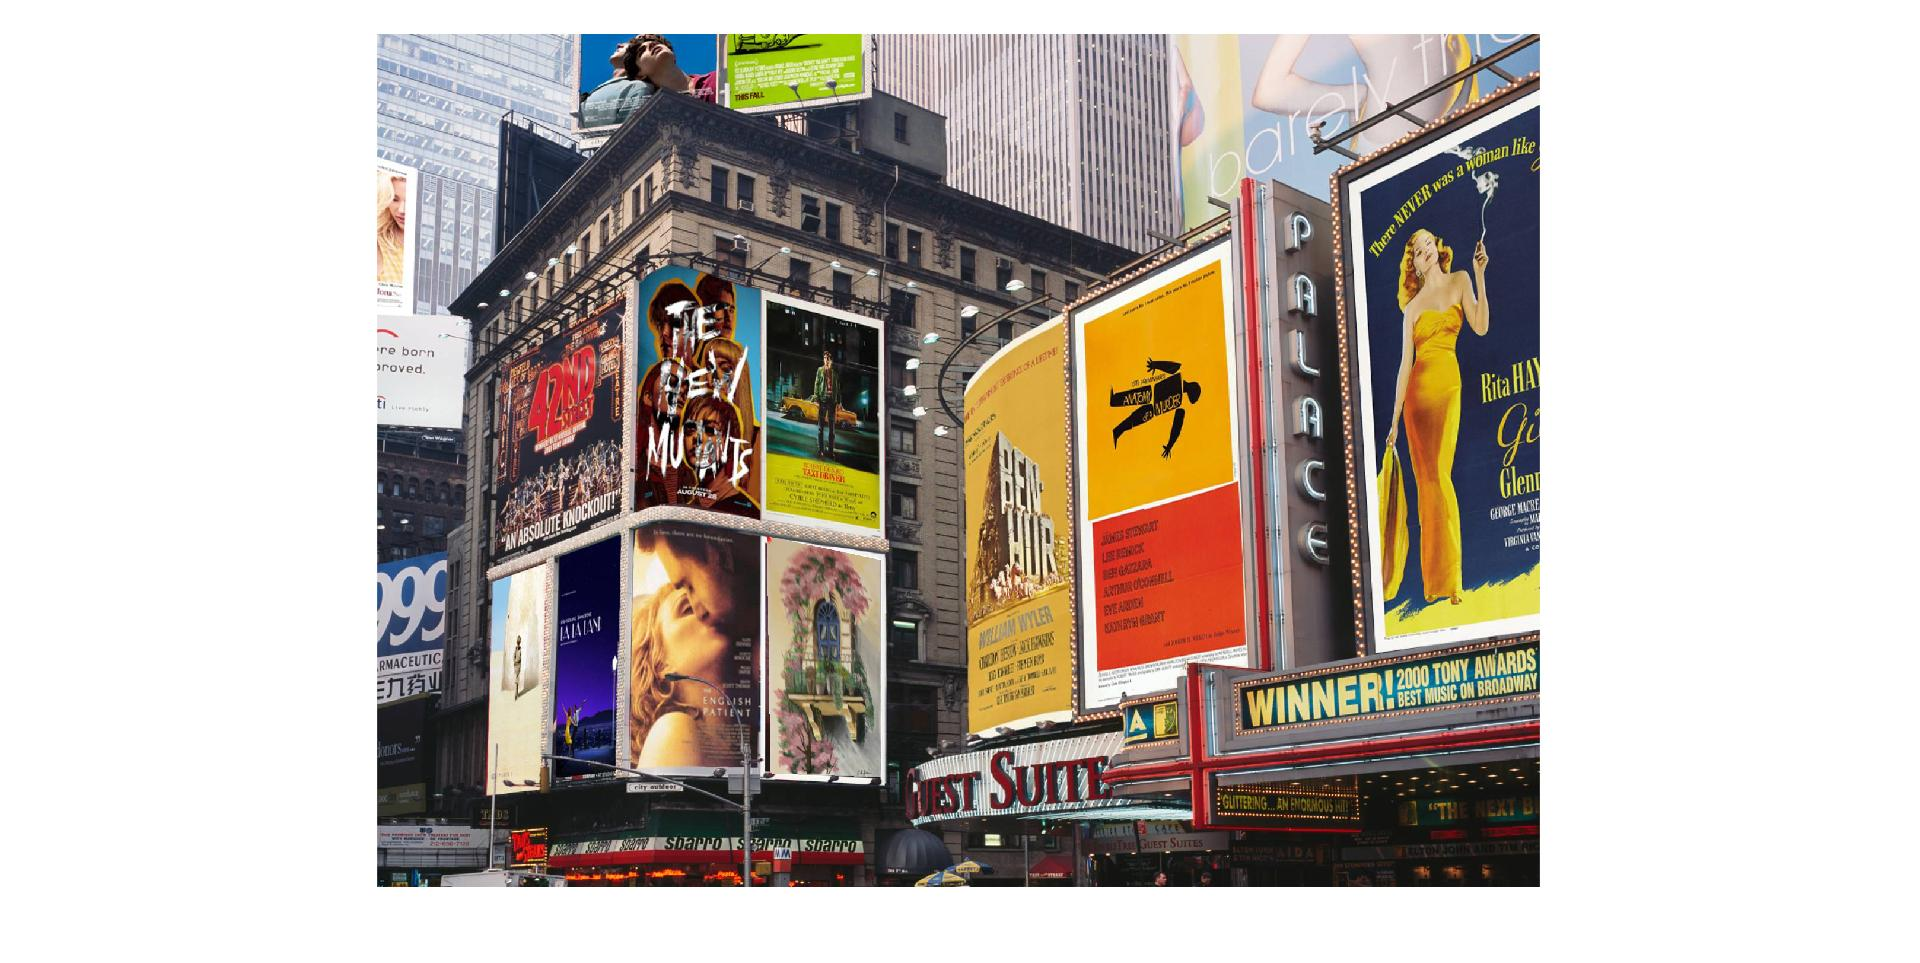
\includegraphics[width=\textwidth]{images/tp_2/incruste2.jpg}
         \caption{Incrusted Image1}
         \label{fig:inc2}
     \end{subfigure}
     \hfill
     \begin{subfigure}[b]{0.3\textwidth}
         \centering
         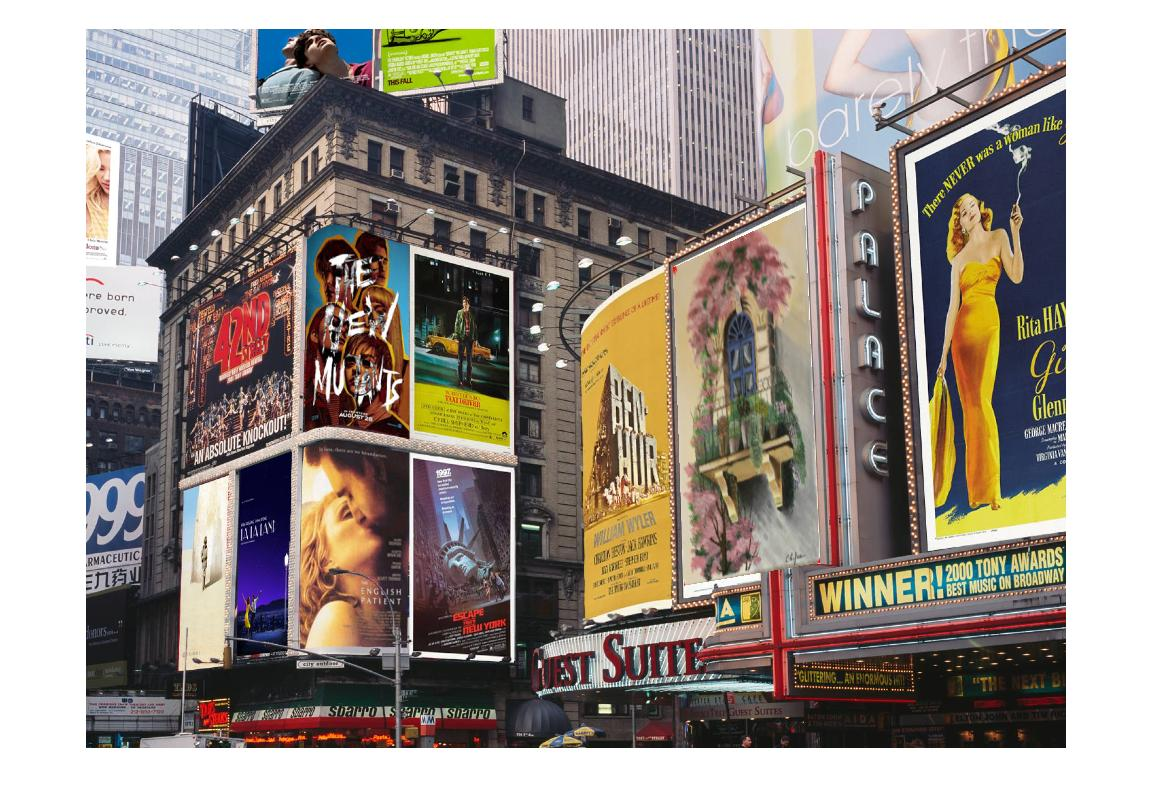
\includegraphics[width=\textwidth]{images/tp_2/incruste3.jpg}
         \caption{Incrusted Image 2}
         \label{fig:inc3}
     \end{subfigure}
     
     \hfill 
        \caption{Images Incrusted}
        \label{fig:inctotal}
\end{figure}

Conversely, the embedding of an image in a scene is performed, in this process the homography matrix was used in the same way, going through the image and pasting the embedding image within the given environment. An example of the embedding of the previously rectified image in a scene is shown in Fig. \ref{fig:inctotal}.

\end{enumerate}




\chapter{Session 3}
The implementation of this section is available in the attached repository at\footnote{\href{https://github.com/GroverAruquipa/3D_Computer_m2}{$https://github.com/GroverAruquipa/3D_Computer_m2$}}.
\begin{enumerate}
    \item \textbf{Acquire two images of an object with distinct faces and with a
transformation between the two cameras easy to find.}
In Fig. \ref{fig:im_tp3}, the images are shown for the right and left, with a translation of $[25\, 5 \, 15]$cm and rotation of 10 degrees around z.

\begin{figure}[H]
     \centering
     \begin{subfigure}[b]{0.4\textwidth}
         \centering
         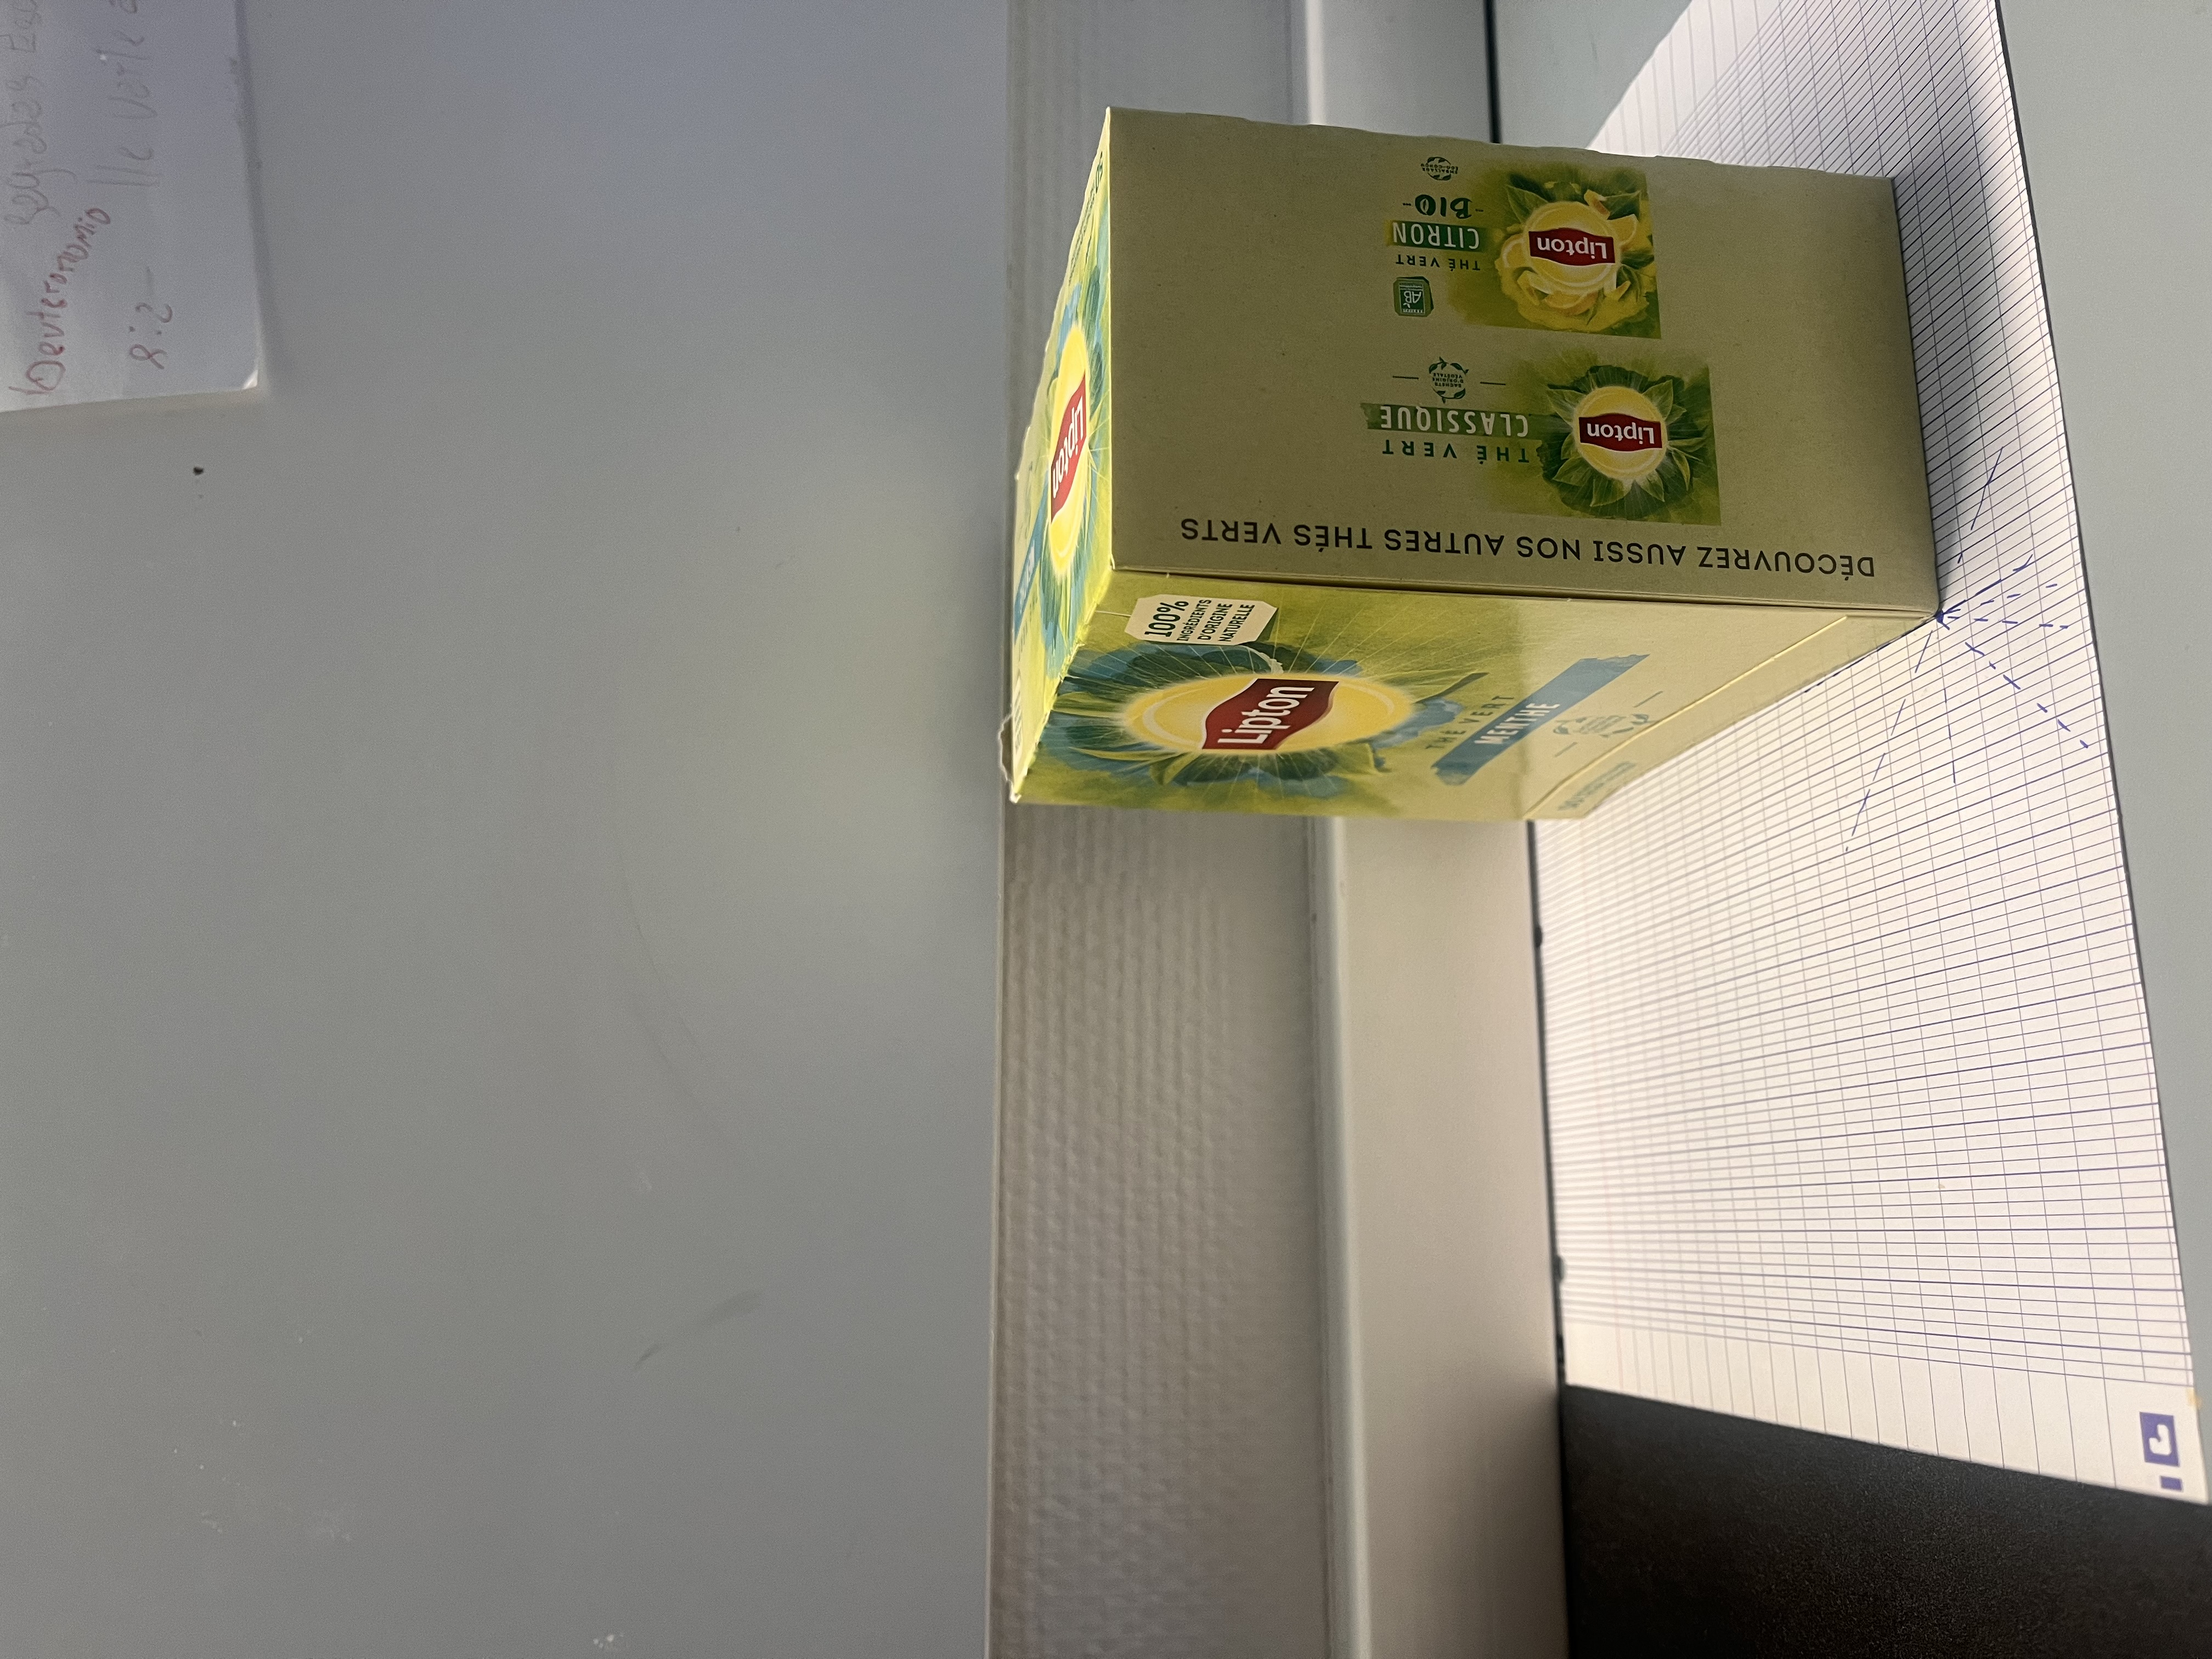
\includegraphics[width=\textwidth]{images/tp_3/img2l.jpg}
             \caption{Right Image}
         \label{fig:fig_rigth}
     \end{subfigure}
     \hfill
     \begin{subfigure}[b]{0.4\textwidth}
         \centering
         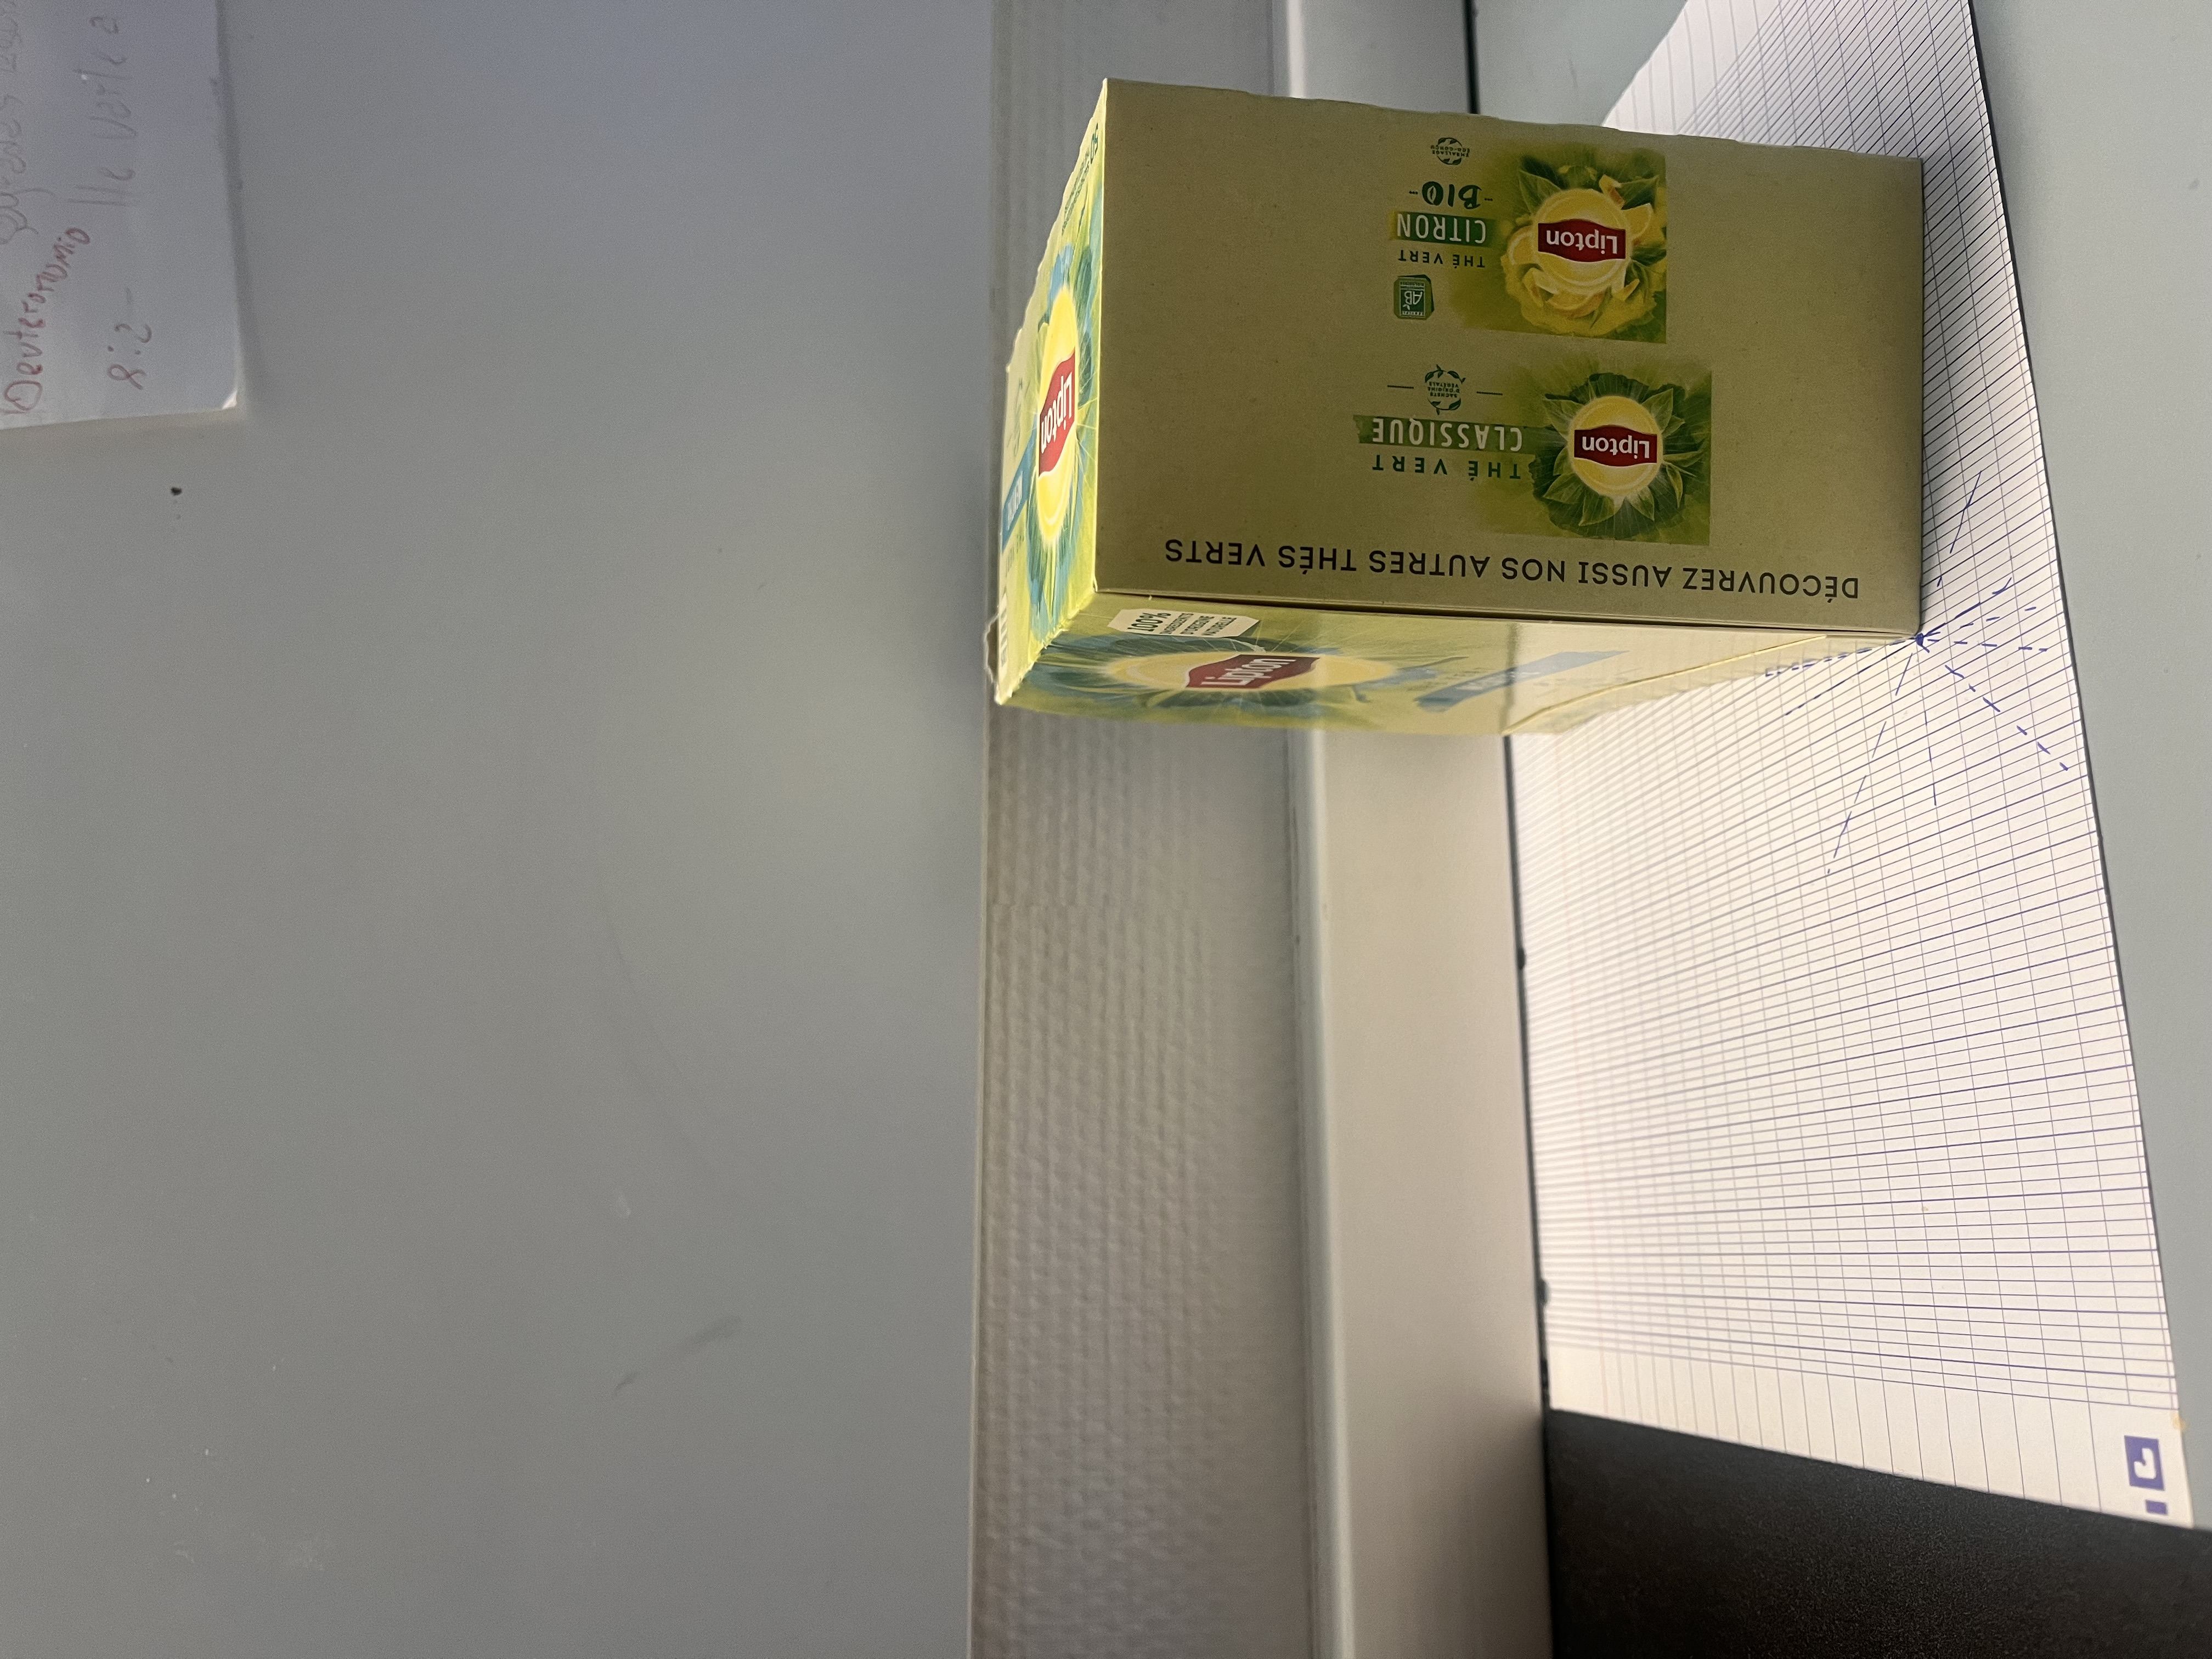
\includegraphics[width=\textwidth]{images/tp_3/img2r.jpg}
         \caption{Left Image}
         \label{fig:fig_left}
     \end{subfigure}
     
     \hfill 
        \caption{Images Acquired}
        \label{fig:im_tp3}
\end{figure}



\item \textbf{Choose 3 (or more) points defining a plane of the observed object to be reconstructed.}\\
In Fig. \ref{fig:fig1_sel} the images are shown with the points selected with different colors.
\begin{figure}[H]
    \centering
    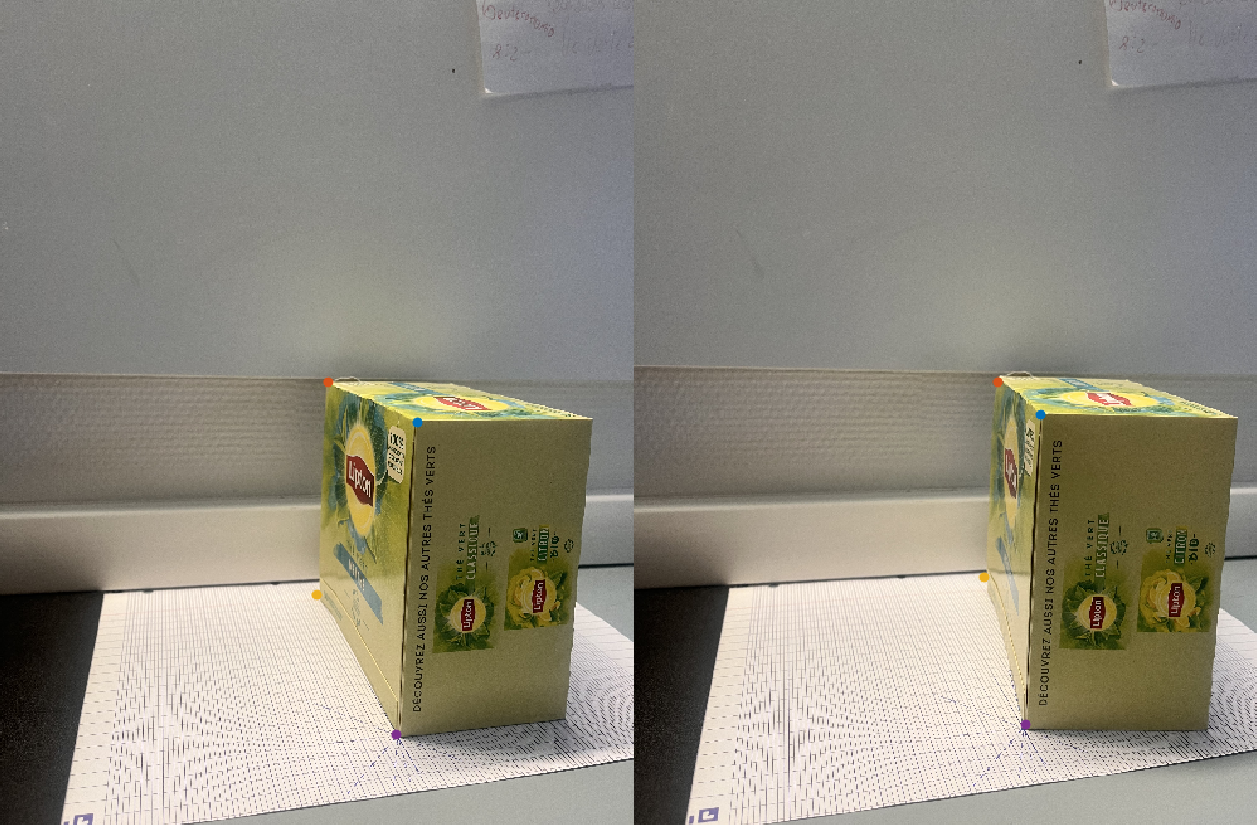
\includegraphics[width=0.5\textwidth]{images/tp_3/4pointsselected.png}
    \caption{Selecting 4 points for each image.}
    \label{fig:fig1_sel}
\end{figure}
\item \textbf{How to solve this equation to arrive at the coordinates gP˜?}\\
In order to solve the proposed equation for the triangulation, once the matrix A has been obtained with the parameters of the camera $K$, the points of each photograph, and the transformation matrix, we proceed to calculate the pseudo inverse, thereby achieving the extraction of the vector $D$, which is reshaped to obtain the solution.
\item \textbf{Implement a function triangulate(K1, K2, Pt1, Pt2, 1Tw,2 Tw) taking as input the intrinsic matrix, the transformation matrix between the two images as well as the corresponding points and
returning the triangulated 3D point.}\\
Below is the triangulation function with the explanation previously made for its calculation of points in 3D.
\begin{lstlisting}[language=Matlab, numbers=none]
    function [pts3D] = triangulate(K1, K2, pts1, pts2, T1_w, T2_w, gama)
    skew1 = [0 -T1_w(3) T1_w(2); T1_w(3) 0 -T1_w(1); -T1_w(2) T1_w(1) 0];
    skew2 = [0 -T2_w(3) T2_w(2); T2_w(3) 0 -T2_w(1); -T2_w(2) T2_w(1) 0];
    imgK = K1;
    %imgKc  
    imgKc = [imgK zeros(3,1)];
    %%% For the image 2 %%%
    imgK2 = K2;
    theta=0; % rotation angle
    alfa=0;
    gama=12*pi/180;
    pt=[0 0 0.25]; % translation
    %transformation matrix 
      T2 = [cos(theta)*cos(gama) -cos(theta)*sin(gama) sin(theta) pt(1); sin(alfa)*sin(theta)*cos(gama)+cos(alfa)*sin(gama) -sin(alfa)*sin(theta)*sin(gama)+cos(alfa)*cos(gama) -sin(alfa)*cos(theta) pt(2); -cos(alfa)*sin(theta)*cos(gama)+sin(alfa)*sin(gama) cos(alfa)*sin(theta)*sin(gama)+sin(alfa)*cos(gama) cos(alfa)*cos(theta) pt(3); 0 0 0 1];
    Ap1=skew1*imgKc;% A matrix is 3x4  for image 1
    clear Ap
    Ap2=skew2*imgKc*T2; % Ap matrix is 3x4 for image 2
    for i=1:size(pts1,1)% for each point
        %skew matrix of pts1 
        skew1=[0 0 pts1(i,2); 0 0 -pts1(i,1); -pts1(i,2) pts1(i,1) 0];
        %skew matrix of pts2
        skew2=[0 0 pts2(i,2); 0 0 -pts2(i,1); -pts2(i,2) pts2(i,1) 0];
        Ap1=skew1*imgKc;
        Ap2=skew2*imgKc*T2;
        % A matrix is 6x4
        A = [Ap1; Ap2];
        [U,S,V] = svd(A);
        % the last column of V is the solution
        pts3D(i,:) = V(:,end);
        pts3D(i,:) = pts3D(i,:)/pts3D(i,4);% normalize the 3D point
    end
%Normalize the 3D points
    %pts3D = pts3D./repmat(pts3D(:,4),1,4);
    %pts3D = pts3D(:,1:3);
end
\end{lstlisting}


\item \textbf{Display in a figure the triangulated points as well as the pose of the cameras used for the calculation.}\\
In Fig. \ref{fig:trian1}, the connected triangulated dots of a face are shown, although they do not form a perfect plane as can be seen, they have a similar similarity, additionally the pose of the camera is shown in Fig. \ref{fig:train2} as a function of the rotation and translation vector used.
\begin{figure}[H]
     \centering
     \begin{subfigure}[b]{0.45\textwidth}
         \centering
         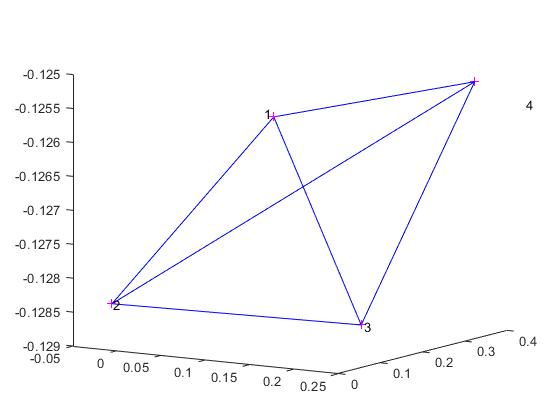
\includegraphics[width=\textwidth]{images/tp_3/points_connected.jpg}
             \caption{Points generated and connected for a plane}
         \label{fig:trian1}
     \end{subfigure}
     \hfill
     \begin{subfigure}[b]{0.45\textwidth}
         \centering
         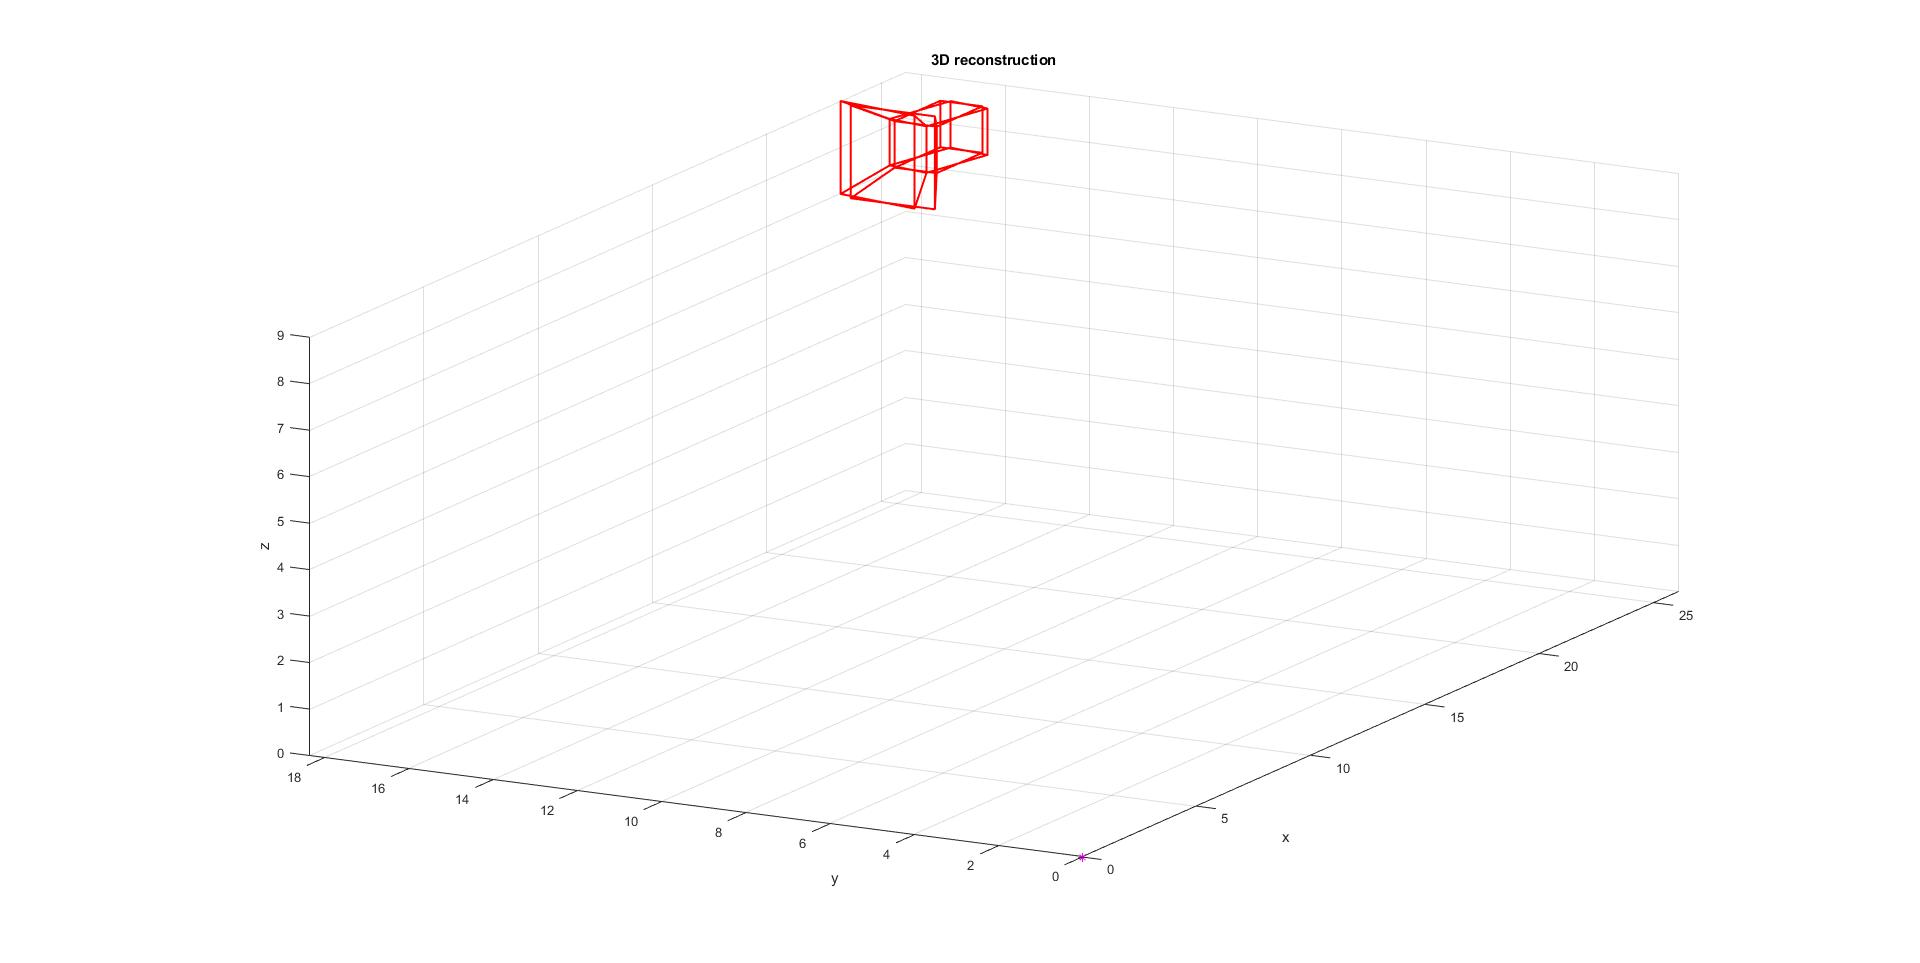
\includegraphics[width=\textwidth]{images/tp_3/cameras.jpg}
         \caption{Plot of the Pose of the cameras}
         \label{fig:train2}
     \end{subfigure}
     
     \hfill
 
        \caption{Triangulation}
        \label{fig:triangulation}
\end{figure}




\item  \textbf{Fill in the plan X variables which consist of the four triangulated corners of face X.}$\,$-$\,$\textbf{Use the calculatePlan function to have a rectangular face if the 4 reconstructed corners do not
are not good enough.} \textit{Two questions inside 1}

For these two questions in 1, the function provided for the calculation of the plane using 3 points was used, with which the projection of point 4 was carried out, in this way being able to carry out the $fill$ operation of the plane, shown in the Fig/ \ref{fig:fig1_filled}.
\begin{figure}[H]
    \centering
    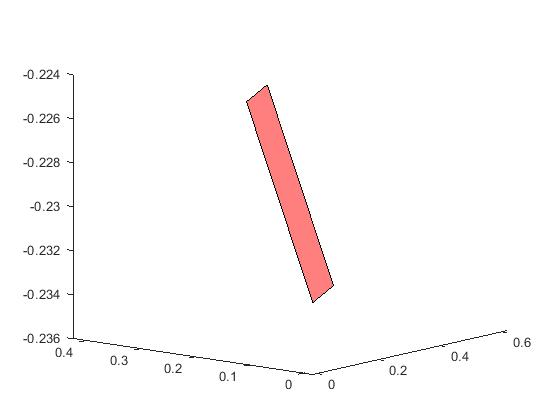
\includegraphics[width=0.5\textwidth]{images/tp_3/plane.jpg}
    \caption{Plane filled.}
    \label{fig:fig1_filled}
\end{figure}
\item \textbf{Choose the triangle points that correspond to the face to be reconstructed.}
Thus, in the same way with the prices of points saved from the different planes, it was carried out in the same previous calculation, entering as results a projection of the points of the object.
\begin{figure}[H]
    \centering
    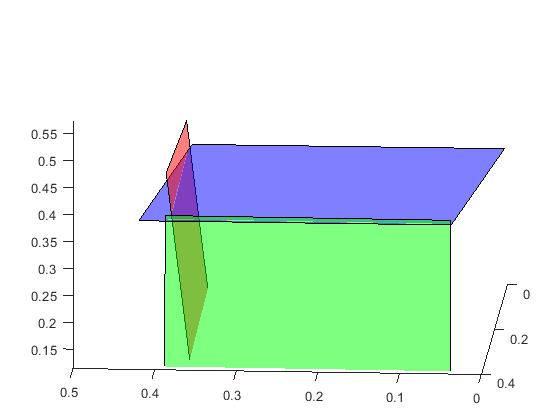
\includegraphics[width=0.5\textwidth]{images/tp_3/faces_points.jpg}
    \caption{Facepoints}
    \label{fig:fig1_face_points}
\end{figure}
\item \textbf{Fill in the p3DX variable which contains the coordinates of each 3D scanX pixel. dX and
dY represents the width and height of the pixel so that the pixel count of p3DX matches that of scanX.}

Finally, the rectification of each plane was carried out in such a way as to move the pixels of each plane within the 3-dimensional project planes, thus finding the projection shown in Fig. \ref{fig:steps}, where the three planes projected in 3D are observed.
\begin{figure}[H]
     \centering
     \begin{subfigure}[b]{0.3\textwidth}
         \centering
         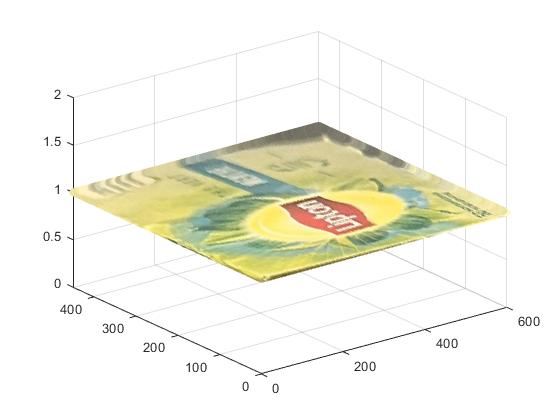
\includegraphics[width=\textwidth]{images/tp_3/face1.jpg}
         \caption{Projection 1}
         \label{fig:face1}
     \end{subfigure}
     \hfill
     \begin{subfigure}[b]{0.3\textwidth}
         \centering
         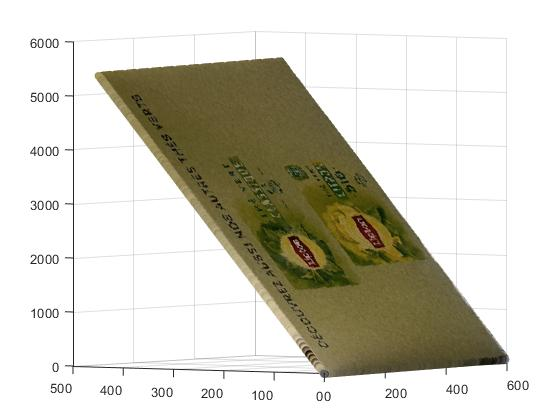
\includegraphics[width=\textwidth]{images/tp_3/face2.jpg}
         \caption{Projection 2}
         \label{fig:face2}
     \end{subfigure}
     \hfill
     \begin{subfigure}[b]{0.3\textwidth}
         \centering
         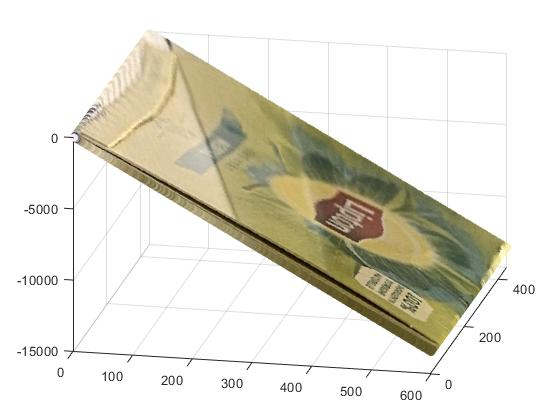
\includegraphics[width=\textwidth]{images/tp_3/face3.jpg}
         \caption{Projection 3}
         \label{fig:face3}
     \end{subfigure}
     \hfill
 
        \caption{Projections and rectifications of the plans in 3D}
        \label{fig:steps}
\end{figure}
\item \textbf{Describe the process of determining the extrinsic parameters of a camera system.}\\
Extrinsic parameters are the geometric parameters of a camera system that describe its location and orientation in space. They are determined by calibrating the camera system using a set of known points or objects. The calibration process involves measuring the distances between the camera and each point or object, and then computing the corresponding camera parameters.

\item \textbf{Describe the principle of operation of epipolar geometry.}

Epipolar geometry is a technique used in computer vision to determine the relative position of two points in a scene. It is based on the fact that, if two points are known, the line between them can be used to determine their relative position. This is because, in a scene, the projection of a point


\item \textbf{What area is it? Cite an example using 3D reconstruction directly like
graphic basis.}

The area is 3D reconstruction. A 3D reconstruction of a human skull can be created from a series of 2D images taken of the skull from different angles.

\end{enumerate}



\chapter{Conclusion}
In these 3 sessions there was an introduction to computer vision in 3 dimensions, different techniques were observed such as the calculation of homography for different scenes and applying photos taken by us, in the same way the camera calibration showed a correct approximation to the calibration in the real world of a camera where the intrinsic parameters are not available and finally an introduction to the 3D reconstruction, where all the results were also fulfilled, thus showing a correct application of the theoretical concepts in the practical part. . Although this laboratory had a slight complexity of application, in future works it will be interesting to be able to explore non-linear methods that help to a much more exact approximation, especially in triangulation and, if possible, hybrid systems with neural networks for noise reduction in the image and the use of dedicated hardware such as a GPU embedded in a platform such as a jetson nanop for navigation and an approach to complex processes such as slam. It ends by noting that all the necessary points for this laboratory were correctly fulfilled.

    
\pagenumbering{gobble}

%printbibliography




\end{document}